% ============================================================================================
% Climbing the Chomsky Hierarchy --- MASTER MANUSCRIPT (InceptLabs self-improvement family).
% Own foundation, PARALLEL to (not built on) the categorical self-revising-discovery line.
% Build: tectonic chomsky_climb.tex . Figures from make_figs.py (figs/fig_cc_*.pdf).
% Results paper: every measured number comes from a logged run in rna_harness/runs/cc_ascent.
% NEVER hand-enter a measured number. Anti-collision with family papers: see POSITIONING.md.
% ============================================================================================
\documentclass[11pt]{article}
\usepackage[margin=1in]{geometry}
\usepackage[utf8]{inputenc}
\usepackage[T1]{fontenc}
\usepackage{textcomp}
\usepackage{amsmath,amssymb,amsthm,amsfonts}
\usepackage{booktabs}
\usepackage{graphicx}
\usepackage{xcolor}
\usepackage{array}
\usepackage{enumitem}
\usepackage{placeins}
\usepackage{tabularx}
\newcolumntype{L}{>{\raggedright\arraybackslash}X}
\usepackage[hidelinks]{hyperref}
\usepackage[numbers,sort&compress]{natbib}
\usepackage{authblk}
\usepackage{caption}
\captionsetup{font=small,labelfont=bf,skip=4pt}
\emergencystretch=1.5em
\graphicspath{{figs/}}

\renewcommand{\topfraction}{0.92}
\renewcommand{\bottomfraction}{0.85}
\renewcommand{\textfraction}{0.06}
\renewcommand{\floatpagefraction}{0.72}
\setcounter{topnumber}{4}\setcounter{bottomnumber}{3}\setcounter{totalnumber}{6}

% (pending/pre-registration markers removed: this is a results paper.)

\newtheorem{theorem}{Theorem}
\newtheorem{proposition}{Proposition}
\newtheorem{lemma}{Lemma}
\newtheorem{corollary}{Corollary}
\newtheorem{definition}{Definition}
\newtheorem{remark}{Remark}

\newcommand{\NESTED}{\ensuremath{\mathcal{L}_{\mathrm{nest}}}}
\newcommand{\PK}{\ensuremath{\mathcal{L}_{\mathrm{pk}}}}
\newcommand{\CF}{\textsc{cf}}
\newcommand{\MCF}{\textsc{mcf}}
\newcommand{\Ocf}{\ensuremath{\Omega_{\mathrm{cf}}}}
\newcommand{\Opk}{\ensuremath{\Omega_{\mathrm{pk}}}}
\newcommand{\Rze}[2]{\ensuremath{\mathcal{R}_{#1}(#2)}}
\newcommand{\match}{\ensuremath{\mathcal{A}_{\mathrm{match}}}}
\newcommand{\umfe}{\ensuremath{\mathcal{A}_{\mathrm{uMFE}}}}
\newcommand{\pfe}{\ensuremath{\mathcal{A}_{\mathrm{pfe}}}}

\title{\textbf{Auditing a Claimed Chomsky-Hierarchy Ascent in RNA Design}\\[3pt]
\large A Two-Sided Capability Certificate for Autonomous Acquisition}
\author[1]{Wenhui Chen\thanks{Corresponding author: \texttt{wenhui.chen@inceptlabs.ai}}}
\affil[1]{InceptLabs-Shanghai}
\date{}

\begin{document}
\maketitle

\begin{abstract}
\noindent Self-improving and self-revising AI-for-science systems increasingly rewrite their own tools,
representations, and search procedures. A central difficulty is telling whether an apparent gain reflects a
\emph{transferable capability} or merely more search, benchmark adaptation, an external tool, or optimization
against a fallible scientific oracle. The evidence usually offered---goodness-of-fit, description-length
gates, significance tests---can attest that a capability \emph{appeared} without establishing that the prior
repertoire could not have produced it. We develop a two-sided, partly \emph{decidable} \emph{audit} of
capability acquisition, and instantiate it where the difficulty axis is not an analogy but a formal fact. RNA
secondary structure realizes a formal-language boundary: pseudoknot-free (nested) structure is context-free
(\CF), while crossing (pseudoknotted) \emph{families} are strictly higher on the Chomsky hierarchy---mildly
context-sensitive, generated by multiple context-free grammars (\MCF)---an established theorem, not a modeling
choice. The audit's core is a two-sided \emph{certificate} of a Chomsky ascent: a self-improving design agent
acquires, autonomously and transferably, the capability to realize crossing (\MCF) targets that its
\CF-verified prior repertoire was confined below. Novelty is relative to the agent's \emph{prior self} on a
real design frontier---not a claim that the capability lies outside the base model, which is neither
measurable nor necessary. The certificate has three operationalized parts: a \emph{positive} side (independent
oracles confirm held-out \MCF{} designs), a \emph{negative} side (a decidable \emph{verifier-confinement}
theorem---the pseudoknot-free folding oracle cannot represent crossing pairs, so the \CF-verified repertoire
scores zero), and an \emph{autonomy} side (an ablation showing the capability is carried by the agent's own
reusable components, not a borrowed solver). We are explicit about an asymmetry the framing must not hide: the
negative side is exact and decidable, whereas the positive side rests on heuristic, model-relative pseudoknot
predictors whose verdict is oracle-dependent and never physical ground truth; we therefore adjudicate it with
a three-predictor panel and abstention-on-disagreement and report it as model-relative. A sealed-commitment
protocol forecloses post-hoc selection. The audit is \emph{complementary} to categorical accounts of
self-revising discovery \citep{selfrevising}: those characterize how a system's representations change, while
ours adjudicates whether a claimed operational capability survives independent verification; it is likewise
distinct from empirical Chomsky-hierarchy evaluation of neural architectures \citep{deletang2023} and from
exact-verifier construction search \citep{funsearch,alphaevolve,alphatensor}. Instantiating it yields our
central---cautionary---result. An agent with an \emph{invented} pseudoknot-design operator (decompose the
target into a context-free skeleton, complete the crossing stem, then repair against a pseudoknot oracle)
solves $43/60$ held-out crossing targets \emph{without} any external solver---seemingly a large autonomous
ascent over a \CF-confined floor of $0/60$. Under the panel this collapses: only $2/43$ survive an
\emph{independent} predictor and $1/60$ is panel-unanimous---the apparent ascent was largely an \emph{oracle
artifact}, the operator having learned to game the predictor it optimized. This is the audit working as
intended: the decidable negative side and the abstaining panel expose oracle-gaming that a one-sided
evaluation would have reported as ``discovery.'' Switching the operator's objective from a single oracle to
\emph{panel agreement} then yields the first panel-robust autonomous crossings we observe: $3$--$8/60$ (mean
$5.0$, five seeds) unanimous across three predictors, versus $\sim\!1/60$ for the gamer and $0/60$ for a
borrowed solver---a small but measurable gain in held-out-oracle robustness above the decidable $0/60$ floor.
The broader lesson for AI4S: self-revision and automated discovery need an \emph{audit layer} that separates
scientific capability from verifier-specific optimization, or a single fallible oracle can dress a $1/60$
robust capability as a $43/60$ discovery.
\end{abstract}

\noindent\textbf{Keywords:} automated scientific discovery; self-improving agents; capability acquisition;
formal language theory; Chomsky hierarchy; RNA inverse design; decidable verification.

\section{Introduction}\label{sec:intro}
Self-improving agents that \emph{claim} new scientific or design capabilities are proliferating, but the
field adjudicates the claim with soft statistics---a reward-model score, a held-out accuracy delta, a
compression/MDL acceptance gate, a $p$-value. None of these separates \emph{acquiring a genuinely new
capability} from \emph{searching more of a fixed space}: a benchmark number rises either way, and a
compression gate accepts a better-fitting model without establishing that the previous model \emph{could
not} have produced the result. Two further confounds are rarely ruled out: the agent may have gotten
\emph{lucky} on a few instances (no transfer), or it may have \emph{borrowed} an external tool (no autonomy).
What is missing is a criterion that is \emph{two-sided}---certifying not only ``can now'' but ``provably
could not before''---and, on at least one side, \emph{decidable}: a verdict computed, not judged.

\paragraph{The opportunity, and why RNA.} One real design problem supplies the substrate such a criterion
needs. In RNA inverse design---find a sequence whose fold is a target secondary structure---the target's
topology is \emph{literally} a position in the Chomsky hierarchy. Nested base pairing is context-free;
crossing base pairing (pseudoknots) is strictly higher, mildly context-sensitive
\citep{rivaseddy2000,nebelweinberg,katosekikasami2006}. Two properties make this the right home. First, the
pseudoknot-free folding oracle \emph{cannot represent} a crossing pair at all: a representational fact that
turns ``the prior repertoire could not'' into a \emph{decidable} statement rather than a failed search.
Second, non-existence of any design for a target (undesignability) admits an exact proof by construction
\citep{zhou2024rigende}. We build the criterion here not because RNA is convenient but because the distinction the
Chomsky hierarchy is founded on---nested vs.\ crossing dependencies---is the same distinction that separates
ordinary RNA structure from pseudoknots.

\paragraph{Thesis.} \emph{A self-improving design agent has achieved a certified Chomsky ascent iff, under a
pseudoknot-aware oracle, it realizes held-out crossing (\MCF) targets via reusable components that survive
ablation, while its prior \CF-verified repertoire is provably confined to nested (\CF) structures. The
negative side is decidable; the positive side is model-relative and adjudicated by an oracle panel.}

\paragraph{Which ``new''?} We are precise about the sense of novelty we certify, because a self-improving
agent runs on a base model that has read the literature, so a capability may be \emph{latent} in the model
even when the agent appears to acquire it. We deliberately do \emph{not} claim novelty \emph{relative to the
base model}---that the capability lies outside its training. That notion is neither measurable (one cannot
audit a model's latent competence) nor necessary: landmark results advance a \emph{frontier}---a faster
matrix multiply, a folded protein---without proving out-of-corpus originality, and all useful discovery
recombines known parts. We certify a different, operational ``new'': the capability is new \emph{relative to
the agent's prior self}---whose repertoire provably could not realize the target (decidable,
\S\ref{sec:formal})---and it crosses a \emph{real, useful frontier} (the $\CF\!\to\!\MCF$ boundary;
pseudoknots are functional structures), \emph{robustly} (surviving an independent oracle panel, not just the
one it optimized) and \emph{autonomously} (no external solver). In an era where models are trained on
everything and evaluations are routinely gamed, this---verified, gaming-resistant capability
acquisition---is the scarce, decision-relevant quantity, not metaphysical originality.

\paragraph{Contributions.}
\begin{enumerate}[leftmargin=1.3em,itemsep=1.5pt]
\item A \emph{two-sided} criterion for capability acquisition (\S\ref{sec:cert})---positive, negative, and
autonomy conditions---that rules out search, luck, and tool-borrowing, replacing soft one-sided gates.
\item A \emph{formalization} of the object a pumping lemma can actually constrain---the agent's
\emph{realizable-target language} $\Rze{\Omega}{\pi}$ (the structures its policy realizes \emph{under an
oracle})---and an \emph{elementary but decidable} confinement fact over it (Prop.~\ref{prop:confine}). The
proposition is deliberately shallow; its content is not mathematical depth but \emph{decidability}---it is
discharged offline, not searched. We add a precise definition of the transferable, autonomous capability, and
\emph{use} (we do not re-prove) the established MCFG-2 characterization as the witness that a realized
crossing target is genuinely mildly-context-sensitive (\S\ref{sec:formal}, App.~\ref{app:proofs}).
\item An explicit treatment of the \emph{certificate's asymmetry} (\S\ref{sec:cert},\ref{sec:oracle}): the
\CF/negative side is exact; the \MCF/positive side is heuristic and oracle-dependent, and we say so and
adjudicate it accordingly---rather than overclaiming a uniform ``exact'' certificate.
\item A clean \emph{separation of two impossibilities} (\S\ref{sec:impossible}): repertoire-confinement (the
ascent's negative side) vs.\ target-undesignability (a distinct, optional predictive capability).
\item The observation, made precise, that RNA topology is native to the Chomsky hierarchy, and a discipline
separating \emph{generative power} (main line) from \emph{folding complexity} (corollary) (\S\ref{sec:cf}).
\item An \emph{empirical demonstration} that the criterion catches oracle-gaming (\S\ref{sec:exp}): an
invented, DesiRNA-free operator scores $43/60$ on held-out crossing targets under a single pseudoknot oracle
but only $1/60$ \emph{panel-unanimous}---a $43\times$ inflation the panel exposes---above a context-free floor
of $0/60$. Re-optimizing the operator for cross-oracle \emph{agreement} then recovers a small panel-robust
ascent ($3$--$8/60$ over five seeds, mean $5.0$, unanimous across three independent predictors)---the honest positive counterpart to the collapse.
\end{enumerate}

\noindent Figure~\ref{fig:arch} shows how these components compose into a single pipeline: a graded target
enters, the agent commits a sealed prediction \emph{before} any oracle is consulted, the pseudoknot-free
ladder and the pseudoknot-aware panel adjudicate the two sides, and the $\pm$solver ablation decides whether
the ascent is the agent's own.

\begin{figure}[t]\centering
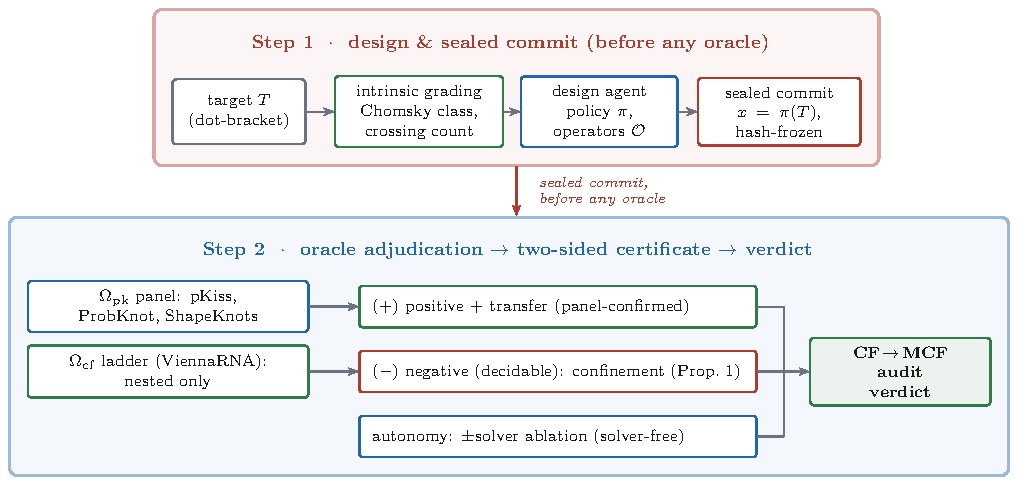
\includegraphics[width=\linewidth]{fig_cc_architecture.pdf}
\caption{\textbf{End-to-end architecture.} A target is graded by its intrinsic Chomsky class and
crossing-stem count and split into a frozen held-out pool; the design agent (policy $\pi$ over reusable
operators, optionally calling an external pseudoknot solver) commits a sealed prediction \emph{before} any
oracle is consulted; adjudication runs the pseudoknot-free ladder $\Ocf$ and the pseudoknot-aware panel
$\Opk$ (abstaining on disagreement); and the two-sided certificate---positive$+$transfer, decidable negative
via Prop.~\ref{prop:confine}, and autonomy under $\pm$solver ablation---issues the verdict. The negative side
is exact; the positive side is model-relative.}\label{fig:arch}
\end{figure}

\paragraph{Scope: what is claimed, demonstrated, and open.} We contribute the foundation, the criterion, its
formalization, the protocol, and \emph{one empirical result}: instantiated on $60$ held-out crossing targets,
the criterion catches an invented operator gaming its oracle---$43/60$ solves under a single predictor
collapse to $1/60$ panel-unanimous, above a $0/60$ context-free floor (\S\ref{sec:exp}, Fig.~\ref{fig:collapse}).
Two things are honestly \emph{not} claimed. (i) A \emph{robust} autonomous ascent: the panel-surviving rate
is $1/60$, so we do not claim the agent has acquired a transferable, model-robust \MCF{} capability---we claim
the sharper, weaker thing, that the instrument \emph{exposes} when an apparent acquisition is an oracle
artifact, and specify in \S\ref{sec:disc} what a robust ascent would require. The algorithm by which an agent
\emph{invents} reusable components remains the object under test, not a contribution we specify. (ii) Any
claim of \emph{scientific discovery of a new design principle}. Table~\ref{tab:claims} maps each claim to its
evidence and status.

\begin{table}[t]\centering\small
\setlength{\tabcolsep}{4pt}\renewcommand{\arraystretch}{1.15}
\caption{Claim--evidence--status. Theorems are proved in App.~\ref{app:proofs}; formal-language facts are
\emph{invoked} from the cited literature; empirical claims are backed by logged runs (\S\ref{sec:exp}).}
\label{tab:claims}
\begin{tabularx}{\linewidth}{@{}p{0.40\linewidth}p{0.31\linewidth}p{0.22\linewidth}@{}}
\toprule
\textbf{Claim} & \textbf{Basis} & \textbf{Status}\\
\midrule
Nested $=$ \CF; crossing families non-\CF (low-dim MCFG); the nested/crossing split maps to the $\CF\!\to\!\MCF$ boundary &
 \citep{rivaseddy2000,nebelweinberg,katosekikasami2006} & invoked; cited\\
A \CF-verified repertoire provably cannot realize a crossing target &
 Prop.~\ref{prop:confine} (oracle output space) & theorem (decidable)\\
The ascent is to \MCF, not a larger CFG & $\PK$ non-CF $+$ MCFG-2 witness
 \citep{nebelweinberg,katosekikasami2006} & theorem $+$ invoked\\
Positive side is model-relative, not exact & oracle-dependence of PK predictors \citep{verifiereconomics}
 & acknowledged; panel+abstain\\
Invented operator solves held-out crossings under \emph{one} oracle & E2 held-out, pKiss & measured: $43/60$\\
That single-oracle rate is largely an \emph{oracle artifact} & independent panel (ProbKnot/ShapeKnots) &
 measured: $1/60$ unanimous\\
Operator needs no external solver (autonomy is \emph{structural}) & $\pm$solver ablation; \CF{} floor &
 measured: $0/60$ floor\\
Repertoire-confinement $\neq$ target-undesignability & \S\ref{sec:impossible} & distinction (theorem)\\
\bottomrule
\end{tabularx}
\end{table}

\section{Background and the Chomsky--RNA Correspondence}\label{sec:bg}
\paragraph{Formal languages and the Chomsky hierarchy.} A grammar generates a language of strings; the
Chomsky hierarchy \citep{chomsky1956,hopcroftullman1979} orders grammars by generative power.
\emph{Context-free grammars} (CFGs) generate exactly the languages recognizable with one stack---
balanced-bracket (Dyck) languages are canonical. The \emph{pumping} and \emph{Ogden} lemmas
\citep{ogden1968,hopcroftullman1979} give necessary conditions for context-freeness, so a word family that
cannot be pumped proves a language is \emph{not} context-free. \emph{Multiple context-free grammars} (MCFGs)
\citep{seki1991mcfg}---equivalent in power to the mildly context-sensitive formalisms of tree-adjoining
grammars and linear context-free rewriting systems \citep{joshi1985tag,vijayshanker1994}---sit just above:
their nonterminals derive \emph{tuples} of substrings placed at several positions, the machinery needed for
\emph{crossing} (copy-like) dependencies one stack cannot track. The MCFG \emph{dimension} bounds how many
substrings a nonterminal coordinates; dimension~2 suffices for the crossing patterns we need. A concrete
anchor fixes the intuition: the Dyck language of balanced brackets is the prototypical context-free language,
accepted by a single pushdown stack that pushes on \verb|(| and pops on \verb|)|. What one stack
\emph{cannot} track are \emph{crossing} dependencies---the textbook non-context-free witnesses are the copy
language $\{\,w\,\#\,w : w\in\Sigma^\ast\}$ and the count language $\{\,a^{n}b^{m}c^{n}d^{m}\,\}$, whose
interleaved $n\!\cdots\!n$ and $m\!\cdots\!m$ constraints force two substrings to grow in lockstep at
separated positions \citep{hopcroftullman1979}. MCFG dimension~2 supplies exactly this: a nonterminal derives
an \emph{ordered pair} of strings that a production may inject at two non-adjacent slots, so the two arms of a
crossing advance together---the minimal machinery above \CF{} and what the crossing families we target
demand. Specific pseudoknot classes are known to sit in low-dimension MCFG subclasses
\citep{katosekikasami2006}; we make no claim that \emph{every} pseudoknot topology is captured at
dimension~2.

\paragraph{RNA secondary structure, folding, inverse design.} An RNA is $x\in\{A,C,G,U\}^n$; a
\emph{secondary structure} is a set $P$ of base pairs (each index paired at most once) drawn as arcs. Pairs
$(i,j),(k,l)$ with $i<k$ \emph{cross} iff $i<k<j<l$; $P$ is \emph{nested} if none cross,
\emph{pseudoknotted} otherwise. A \emph{folding oracle} maps a sequence to a structure under a thermodynamic
model---from base-pair maximization \citep{nussinov1980} through minimum-free-energy dynamic programming
\citep{zuker1981} and the equilibrium partition function \citep{mccaskill1990} to the ViennaRNA package
\citep{hofacker1994,lorenz2011}. The standard minimum-free-energy oracle (ViennaRNA, Turner parameters),
written \Ocf, is \emph{pseudoknot-free}: its output space is exactly the nested structures, and it
\emph{cannot represent} a crossing pair. \emph{Inverse design}---given target $T$, find $x$ with
$\mathrm{fold}(x)=T$---is a mature task with heuristic \citep{busch2006inforna}, ensemble-defect
\citep{zadeh2011nupack}, learned \citep{runge2019learna}, ensemble-optimization \citep{zhou2023samfeo}, and
pseudoknot-capable \citep{kleinkauf2015antarna,wirecki2025desirna} solvers. Pseudoknot-aware \emph{prediction}
oracles \Opk{}---pKiss \citep{janssen2015pkiss}, ProbKnot \citep{bellaousov2010probknot}, ShapeKnots
\citep{hajdin2013shapeknots}, in the lineage of \citep{rivas1999pknots,akutsu2000}---can output crossings but
are \emph{heuristic}, not biophysical ground truth. Pseudoknot-free folding is polynomial; pseudoknotted
folding is NP-complete \citep{lyngso2000pknot,lyngso2004,condon2004}, and inverse design is NP-hard even in the minimal
base-pair-maximization model \citep{bonnet2020hard}. The sequence$\to$structure map is many-to-one, with
large neutral networks \citep{schuster1994,aguirre2011}; \emph{undesignability}---no sequence realizes
$T$---is provable by exhibiting, for every candidate, a rival structure at least as favorable
\citep{zhou2024rigende,zhou2025motifs}.

\paragraph{The verifier ladder (a reused instrument).} Our companion work \citep{verifiereconomics} turns
``solved'' into a nested family of decidable predicates on one target,
$\match\supseteq\umfe\supseteq\pfe$, under \Ocf, with a separate pseudoknot-aware branch for crossing
targets. We reuse this as the \emph{adjudicating instrument} our certificate calls, and stake an orthogonal
thesis (capability-class acquisition, not verifier over-acceptance). Crucially, that companion also
\emph{measured the oracle-dependence of the pseudoknot verdict}: the fraction of state-of-the-art
pseudoknot designs judged ``formed'' swings across predictors (pKiss/ProbKnot/ShapeKnots), a
$[\,15,60\,]\%$ envelope. We carry this fact into our positive-side design (\S\ref{sec:oracle}).

\subsection{RNA Topology Is Native to the Chomsky Hierarchy}\label{sec:cf}
That biological sequence structure is fruitfully read as a formal language is a long tradition
\citep{searls1992,searls2002}. Nested arcs are balanced brackets---context-free, generated by the RNA
stochastic context-free grammar $S\to(\,S\,)\,S\mid\mathord{.}\,S\mid\varepsilon$, the classical model of RNA
folding \citep{rivaseddy2000,durbin1998}, with SCFGs the standard nested-RNA model
\citep{sakakibara1994,knudsenhein1999,dowelleddy2004} and thermodynamic pseudoknot folders operating over
the mildly-context-sensitive class \citep{reedergiegerich2004}. Crossing arcs are provably \emph{not}
context-free---an Ogden-lemma argument on the interleaved
crossing dependencies rules out any CFG \citep{nebelweinberg}---and are captured by an MCFG of dimension
$\le 2$; the canonical pseudoknot grammar of \citet{rivaseddy2000} was shown to be exactly such
\citep{katosekikasami2006}. The pseudoknot-free/pseudoknot split that a design pipeline already treats as two
verifier branches therefore \emph{coincides} with the $\CF\!\to\!\MCF$ boundary (Fig.~\ref{fig:hierarchy}).

\begin{figure}[t]\centering
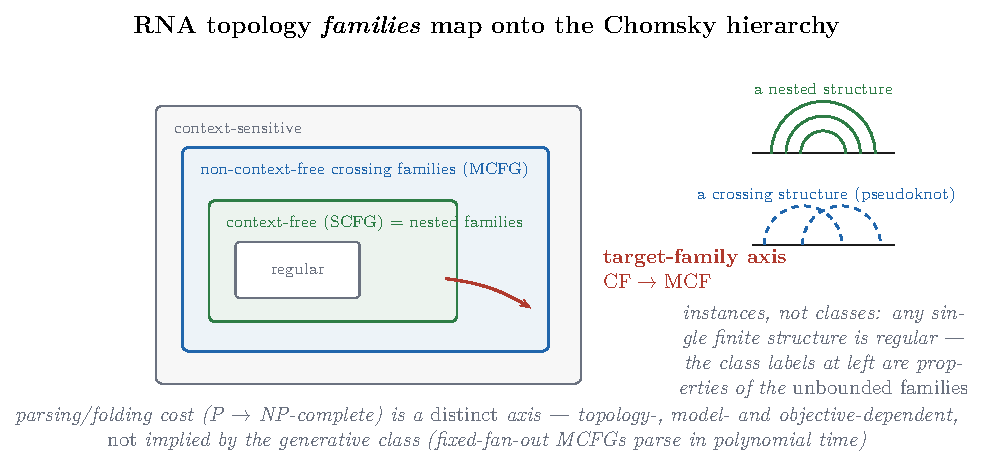
\includegraphics[width=0.86\linewidth]{fig_cc_hierarchy.pdf}
\caption{\textbf{RNA topology maps onto the Chomsky hierarchy.} Nested base pairs are context-free (SCFG);
crossing pairs (pseudoknots) are, as unbounded families, non-\CF{} and admit mildly context-sensitive (MCFG)
grammars, provably above \CF. The climb is the $\CF\!\to\!\MCF$ jump; folding complexity (P$\to$NP-complete)
is a corollary of the class, not the main line.}\label{fig:hierarchy}
\end{figure}

\paragraph{Why one stack fails, concretely.} Reading a strand $5'\!\to\!3'$, the nested grammar
$S\to(\,S\,)\,S\mid\mathord{.}\,S\mid\varepsilon$ folds with a single stack: each opening base is pushed and
its partner pops it, and well-nesting guarantees the most-recently-opened pair closes first
(last-in-first-out). A canonical H-type pseudoknot violates precisely this discipline. Written in dot-bracket
form with two pair classes, $(((([[[[))))]]]]$, the square-bracket stem opens while the round-bracket pairs
are still unclosed and must be remembered \emph{past} the closing of the round stem---a second, independent
stack. This is the copy-language pattern, not the Dyck pattern: an Ogden-lemma argument on the interleaved
dependencies rules out every CFG \citep{nebelweinberg}, whereas an MCFG carrying the two stems as a
coordinated pair of substrings generates it at dimension~2 \citep{katosekikasami2006}. The two verifier
branches a design pipeline already maintains---pseudoknot-free folding versus pseudoknot-aware
prediction---thus do not merely differ in difficulty; they \emph{straddle a generative-class boundary}. We
develop this example formally, as the smallest target that certifies the ascent, in \S\ref{sec:formal}.

\paragraph{Generative power is the main line; complexity is a corollary.} The Chomsky hierarchy measures
\emph{generative power} (which structures a grammar produces); computational complexity measures the
\emph{cost} of parsing/folding. Pseudoknotted folding is NP-complete and inverse design is NP-hard
\citep{lyngso2000pknot,bonnet2020hard}, but that hardness is a downstream corollary of the language class, not our object.
Our sole main-line quantity is the generative jump $\CF\!\to\!\MCF$; complexity claims appear only as
consequences, always with their energy-model qualifier. This avoids conflating an expressiveness boundary
with a complexity boundary.

\section{The Two-Sided Ascent Certificate}\label{sec:cert}
Each target receives an \emph{intrinsic} difficulty grade---by crossing-stem count and Chomsky class---never
conditioned on which targets the agent solves, avoiding survivorship bias. We split crossing (\MCF) targets
by grade into a training pool and a \emph{frozen held-out} pool.

\begin{definition}[Certified Chomsky ascent]\label{def:cert}
A capability gain is a \emph{certified ascent} iff all three hold:
\begin{description}[leftmargin=1.4em,itemsep=1pt]
\item[\textnormal{(1) Positive $+$ transfer.}] On \emph{held-out} \MCF{} targets, the agent produces designs
that a pseudoknot-aware oracle panel confirms fold to the target's crossing pair set, at a rate above zero
and spread across targets (not concentrated on one).
\item[\textnormal{(2) Negative (decidable).}] The agent's \emph{prior} repertoire, verified under the
pseudoknot-free oracle \Ocf, provably cannot realize those targets: \Ocf's output space is exactly the
nested structures (Prop.~\ref{prop:confine}), so its realizable-target language contains no crossing target.
\item[\textnormal{(3) Autonomy.}] The capability is carried by the agent's own reusable components, not by
delegating to an external pseudoknot solver: removing the external solver leaves held-out performance
essentially unchanged, and the reusable components are \emph{learned} (reused with positive lift) and
\emph{decisive} (ablating them collapses the gain).
\end{description}
\end{definition}
\noindent Writing $\widehat p^{\mathrm{panel}}_{\bullet}(\mathcal D_{\mathrm{ho}})$ for the held-out
panel-unanimous rate, $\Delta\mathcal O=\mathcal O_{\mathrm{after}}\!\setminus\!\mathcal O_{\mathrm{before}}$
for the reused components, and $\ominus$ for ablation, the three conditions are
\begin{equation}\label{eq:cert}
\underbrace{\widehat p^{\mathrm{panel}}_{\mathrm{after}}(\mathcal D_{\mathrm{ho}})>0}_{\text{(1) positive}+\text{transfer}}
\ \wedge\
\underbrace{\Rze{\Ocf}{\pi_{\mathrm{before}}}\cap\PK=\varnothing}_{\text{(2) negative: a theorem (Prop.~\ref{prop:confine})}}
\ \wedge\
\underbrace{\widehat p^{-\mathrm{solver}}_{\mathrm{after}}\!\approx\widehat p_{\mathrm{after}}
\ \wedge\ \widehat p^{\,\ominus\Delta\mathcal O}_{\mathrm{after}}=0}_{\text{(3) autonomy: solver-free and $\Delta\mathcal O$-decisive}}\,.
\end{equation}
Only conjunct~(2) is decidable and discharged before any run; (1) and~(3) are measured and model-relative.

\paragraph{What each side rules out.} The positive side alone is \emph{search} (a benchmark can rise from
exploration) and does not exclude \emph{luck} (which the transfer/spread requirement addresses). The
negative side converts ``can now'' into ``could not before'', excluding the explanation that the target was
always in reach. The autonomy side excludes \emph{borrowing}: ``solved a pseudoknot'' must not mean ``called
a pseudoknot solver.'' Only the conjunction certifies capability \emph{acquisition}. These four
alternatives---search, luck, benchmark overfitting, and borrowing---are exactly the ones that soft,
one-sided evidence leaves open: a rising reward-model score or held-out delta is equally consistent with
reward over-optimization and specification gaming \citep{skalse2022,gao2023overopt,amodei2016concrete}, and a
compression- or fit-based acceptance gate endorses a better-fitting model without excluding that the prior
model could have produced the result too. The negative side is what shuts that last door. The trichotomy is
deliberate and parallels the retrieval/search/discovery distinction drawn categorically by
\citet{selfrevising}: our condition~(1) rules out retrieval and mere search, (3) rules out borrowing, and
(2)---the decidable impossibility of the prior repertoire---is what earns the word \emph{acquisition}.
Table~\ref{tab:anatomy} sets the three sides against the alternative each is there to neutralize.

\begin{table}[t]\centering\small
\caption{\textbf{Anatomy of the certificate.} Each side neutralizes a distinct alternative to genuine
capability acquisition; the three differ in what adjudicates them and whether the verdict is exact. Only the
conjunction is load-bearing.}
\label{tab:anatomy}
\begin{tabularx}{\linewidth}{@{}l L L l@{}}
\toprule
Side & Neutralizes & Instrument & Verdict \\
\midrule
(1) Positive $+$ transfer & search; one-off luck & pseudoknot-aware oracle panel on \emph{held-out} \MCF{}
targets, spread across targets & model-relative \\
(2) Negative & ``could always have'' (target already in reach) & Prop.~\ref{prop:confine}: output space of
\Ocf{} $=$ nested structures, contains no crossing target & exact, decidable \\
(3) Autonomy & borrowing an external solver & $\pm$solver ablation; reuse that is \emph{learned}
(lift${}>{}0$) and \emph{decisive} (ablation collapses the gain) & empirical \\
\bottomrule
\end{tabularx}
\end{table}

\paragraph{The certificate is asymmetric---and we say so.} The negative side is \emph{exact and decidable}:
it rests on the representational limit of \Ocf{} (Prop.~\ref{prop:confine}), a computed fact. The positive
side is \emph{not} exact: \Opk{} is a heuristic, model-relative predictor whose verdict is oracle-dependent
(\S\ref{sec:bg},\ref{sec:oracle}). We therefore do not claim a uniformly ``exact'' certificate; we claim a
decidable negative side and a model-relative, panel-adjudicated positive side, and we report the positive
rate with its cross-oracle envelope (\S\ref{sec:oracle}). This asymmetry is a feature to be stated, not a
gap to be hidden.

\paragraph{Sealed-commitment protocol.} For each held-out target the agent commits, \emph{before} any oracle
is consulted, a hash-frozen prediction (a candidate sequence, or an explicit abstention/undesignability
claim, \S\ref{sec:impossible}); only then is the panel run. This makes each prediction risky and forecloses
post-hoc selection of favorable cases. This operationalizes a Lakatosian \emph{risky prediction}
\citep{popper1959,lakatos1978}: by committing---including an explicit undesignability claim
(\S\ref{sec:impossible}) that the oracle is free to refute---before the verdict is known, each held-out
target becomes a genuine opportunity to be wrong, and no result can be rescued by choosing the favorable
cases afterward. It is the design-time analogue of pre-registration, and of recent agentic falsification
loops \citep{huang2025popper,liu2024aigs}, but with an \emph{exact} refuter on the negative side rather than
a statistical one. Figure~\ref{fig:cert} summarizes the certificate.

\paragraph{The certification procedure and its soundness.} Certifying an ascent on a held-out pool
$\mathcal D_{\mathrm{ho}}$ runs five steps: \emph{(i)} pre-screen $\mathcal D_{\mathrm{ho}}$ for designability
(\S\ref{sec:exp}), moving intrinsically unrealizable targets to the undesignability axis
(\S\ref{sec:impossible}); \emph{(ii)} discharge the negative side offline by testing
$\mathcal D_{\mathrm{ho}}\subseteq\PK$ (Prop.~\ref{prop:confine}), which fixes the \CF{} floor at $0$;
\emph{(iii)} for each $T$, hash-commit $\pi_{\mathrm{after}}(T)$ (or an abstention) \emph{before} any oracle
call; \emph{(iv)} adjudicate by the panel-unanimous rule with abstention (\S\ref{sec:oracle}); \emph{(v)}
ablate---remove the external solver, then remove $\Delta\mathcal O$---and recompute. With $\mathbf 1[\cdot]$
the indicator and $\pi^{-s},\pi^{\ominus\Delta\mathcal O}$ the solver-removed and component-ablated policies,
the reported quantities are
\begin{equation}\label{eq:metrics}
  \widehat p_{\Omega}(\mathcal D)=\frac{1}{|\mathcal D|}\sum_{T\in\mathcal D}\mathbf 1\!\left[\Omega(\pi(T))=T\right],
  \qquad
  g_{\mathrm{aut}}=\widehat p_{\Opk}-\widehat p^{\,-s}_{\Opk},
  \qquad
  g_{\mathrm{tr}}=\widehat p_{\Opk}(\mathcal D_{\mathrm{train}})-\widehat p_{\Opk}(\mathcal D_{\mathrm{ho}}),
\end{equation}
the panel-unanimous held-out rate, the autonomy gap, and the transfer gap.

\begin{remark}[Soundness rationale; not a formal theorem]\label{prop:sound}
This is a design rationale, not a proved theorem: we do not formalize an adversary model over policy/oracle
pairs. Informally, if Eq.~\eqref{eq:cert} holds under the sealed-commitment protocol, each conjunct targets a
distinct confounder: \emph{search} and one-off \emph{luck} by a held-out, target-spread positive rate
committed before adjudication; \emph{``could always have''} by the decidable emptiness
$\Rze{\Ocf}{\pi_{\mathrm{before}}}\cap\PK=\varnothing$; \emph{benchmark overfitting} by transfer
($g_{\mathrm{tr}}$ small) to targets disjoint from those forming $\Delta\mathcal O$; and \emph{borrowing} by a
near-zero autonomy gap $g_{\mathrm{aut}}\!\approx\!0$ with $\Delta\mathcal O$-decisiveness
$\widehat p^{\,\ominus\Delta\mathcal O}\!=\!0$. The conjunction is \emph{non-redundant} in the informal sense
that dropping~(2) readmits ``could always have'', dropping~(3) readmits borrowing, and dropping~(1) leaves
nothing measured; we make no claim of formal minimality.
\end{remark}
\noindent The verdict is a demarcation, not a probability: conjunct~(2) is a theorem (Prop.~\ref{prop:confine}),
whereas (1) and~(3) are model-relative measurements whose uncertainty we quantify (\S\ref{sec:exp}, Table~\ref{tab:sep}).

\begin{figure}[t]\centering
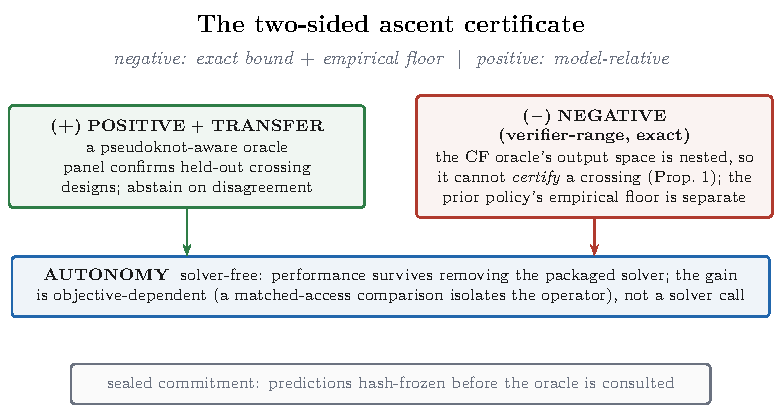
\includegraphics[width=0.96\linewidth]{fig_cc_certificate.pdf}
\caption{\textbf{The two-sided certificate.} Positive side (model-relative, panel-adjudicated): the oracle
panel confirms held-out \MCF{} designs and transfer. Negative side (exact, decidable): the pseudoknot-free
oracle cannot represent crossings (Prop.~\ref{prop:confine}). Autonomy: reusable components survive solver
removal and ablation. Sealed commitment freezes predictions.}\label{fig:cert}
\end{figure}

\subsection{The Positive Side Is Model-Relative}\label{sec:oracle}
The negative side of the certificate is exact (Prop.~\ref{prop:confine}); the positive side is not, and
honesty requires foregrounding the difference. A ``formed pseudoknot'' verdict comes from a \emph{heuristic}
predictor over a restricted pseudoknot class, not from biophysical ground truth, and the verdict is
\emph{oracle-dependent}: our companion measured that the fraction of state-of-the-art pseudoknot designs
judged to form their target swings across predictors---a $[\,15,60\,]\%$ envelope over pKiss, ProbKnot, and
ShapeKnots, with only fair pairwise agreement \citep{verifiereconomics} (Fig.~\ref{fig:oracle}). The disagreement has a mechanistic source rather than
being mere noise: the three predictors cover different pseudoknot subclasses and optimize different
objectives---pKiss enumerates H-type and kissing-hairpin motifs under a heuristic folding model
\citep{janssen2015pkiss}, ProbKnot assembles maximum-expected-accuracy pairs from a partition function
\citep{bellaousov2010probknot}, and ShapeKnots is designed to fold under experimental probing constraints
\citep{hajdin2013shapeknots}---so a single-predictor rate is not just noisy but systematically class-biased.
A positive rate reported under a single lenient predictor would therefore be an oracle artifact, not a
capability. Abstaining when the panel disagrees is the conservative reading: it declines to convert a
modeling artifact into a claimed capability.

\begin{figure}[t]\centering
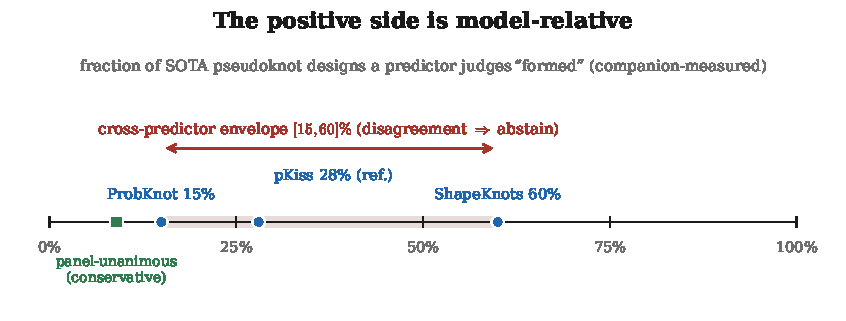
\includegraphics[width=0.82\linewidth]{fig_cc_oracle.pdf}
\caption{\textbf{The positive side is model-relative.} The fraction of state-of-the-art pseudoknot designs
judged to ``form'' their target swings across predictors---a $[\,15,60\,]\%$ envelope over ProbKnot, pKiss,
and ShapeKnots, measured in the companion \citep{verifiereconomics}. We report the conservative
panel-unanimous rate as primary, pKiss as reference, and the full envelope, abstaining where predictors
disagree. Values are companion-measured; no rate is fixed in this manuscript.}\label{fig:oracle}
\end{figure}

We adjudicate the positive side accordingly. A held-out crossing target counts as realized only under an
explicit rule, and we report all three: (i) \emph{panel-unanimous}---all three predictors confirm the exact
crossing pair set---as the \emph{primary} rate; (ii) the \emph{reference} (pKiss) rate; and (iii) the
cross-predictor \emph{envelope} $[\min,\max]$. Targets on which predictors disagree are \emph{abstained}
rather than counted either way. Thus the certificate is asymmetric by construction: a decidable, exact
negative side and a model-relative, panel-adjudicated, abstaining positive side. We claim exactly this---not
a uniformly ``exact'' certificate---and we regard stating the asymmetry as part of the contribution, since
it is precisely the property that a soft-statistic evaluation leaves implicit.

\section{Formalization: the Realizable-Target Language}\label{sec:formal}
A pumping lemma constrains \emph{languages of structures}; an agent manipulates \emph{sequences}. The object
the lemma can act on is therefore not the agent's operators but the set of \emph{target structures the agent
realizes under an oracle}. Making this precise fixes a category error latent in a naive ``operators place
pairs'' account: an operator edits a \emph{sequence}, and whether the result is nested or crossing is a
property of the \emph{fold}, decided by the oracle---not of the operator.

\paragraph{Policies, oracles, and the realizable-target language.}
\begin{definition}[Structures, oracles, policies]\label{def:setup}
Fix $\Sigma=\{\mathrm A,\mathrm C,\mathrm G,\mathrm U\}$ and let $\mathcal T=\bigcup_n\mathcal T_n$ be the
dot-bracket structures, partitioned into the \emph{nested} language $\NESTED$ (no two base pairs cross) and
the \emph{crossing} language $\PK=\mathcal T\setminus\NESTED$. A \emph{folding oracle} is a length-preserving
map $\Omega:\Sigma^\ast\!\to\mathcal T$; a \emph{design policy} is a length-preserving map
$\pi:\mathcal T\!\to\Sigma^\ast$, realized by a search over a repertoire of reusable components $\mathcal O$.
The \emph{realizable-target language} of $\pi$ under $\Omega$ and the \emph{designable set} of $\Omega$ are
\begin{equation}\label{eq:realizable}
  \Rze{\Omega}{\pi}=\{\,T\in\mathcal T:\Omega(\pi(T))=T\,\},\qquad
  \mathcal D_\Omega=\operatorname{im}\Omega=\{\,T:\exists\,x\in\Sigma^\ast,\ \Omega(x)=T\,\}.
\end{equation}
$\Rze{\Omega}{\pi}$ is a language over dot-bracket strings---the object a Chomsky-class statement must range
over, since a pumping lemma constrains languages of \emph{structures}, not the sequence edits an operator
performs.
\end{definition}

\begin{lemma}[Realizability is capped by the oracle range]\label{lem:bound}
For every policy $\pi$ and oracle $\Omega$, $\ \Rze{\Omega}{\pi}\subseteq\mathcal D_\Omega=\operatorname{im}\Omega$,
independently of the policy's search budget or repertoire.
\end{lemma}
\begin{proof}
If $T\in\Rze{\Omega}{\pi}$ then $T=\Omega(\pi(T))$, so $T$ is in the image of $\Omega$; i.e.\
$T\in\operatorname{im}\Omega=\mathcal D_\Omega$. The bound quantifies over \emph{all} $\pi$, so no amount of
search enlarges $\Rze{\Omega}{\pi}$ beyond $\operatorname{im}\Omega$.
\end{proof}
\noindent Lemma~\ref{lem:bound} is the engine of the negative side: it makes confinement a property of the
\emph{oracle's representation}, not of any operator, and reduces Prop.~\ref{prop:confine} to computing
$\operatorname{im}\Ocf$.

\paragraph{Where this object sits in designability theory.} $\Rze{\Omega}{\pi}$ is bounded above by the set
of \emph{designable} structures under $\Omega$---those admitting at least one sequence that folds to
them---and so inherits the sharp non-uniformity of the sequence-to-structure map: designable structures form
vast neutral networks, while many structures are realized by no sequence at all
\citep{schuster1994,aguirre2011}. Its extreme, \emph{undesignability}---no sequence realizes $T$ under the
energy criterion---is provable by construction \citep{zhou2024rigende} and is the complement of the designable
set. This carries a protocol consequence we act on in \S\ref{sec:exp}: a held-out crossing pool must be
pre-screened for designability, so that an intrinsically unrealizable target is scored as an impossibility
(\S\ref{sec:impossible}) rather than mistaken for a capability failure. The realizable-target language is
thus the intersection of what is \emph{designable in principle} and what the policy $\pi$ \emph{actually
finds}; a certified ascent is a claim about the second factor, made only over targets the first factor
admits (Fig.~\ref{fig:lang}).

\begin{figure}[t]\centering
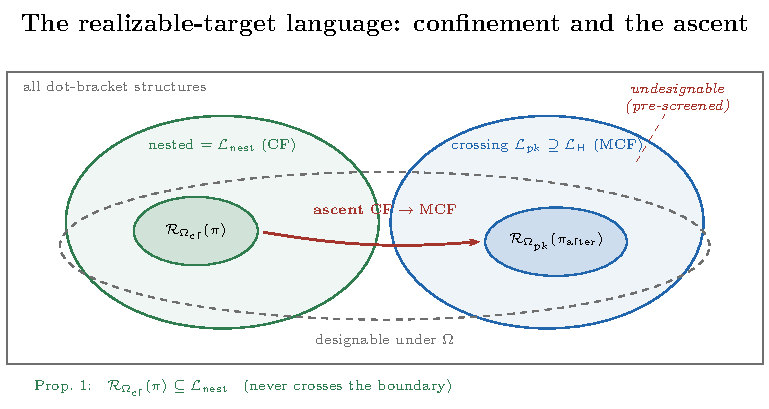
\includegraphics[width=0.9\linewidth]{fig_cc_language.pdf}
\caption{\textbf{The realizable-target language, confinement, and the ascent.} Nested structures form a
context-free region $\NESTED$ and crossing structures a disjoint, strictly higher region $\PK$; the
designable set (dashed) is the subset realized by some sequence. Under the pseudoknot-free oracle, the
realizable-target language $\Rze{\Ocf}{\pi}$ is confined to $\NESTED$ (Prop.~\ref{prop:confine}) and cannot
enter $\PK$; a certified ascent moves $\Rze{\Opk}{\pi_{\mathrm{after}}}$ into the designable part of $\PK$,
while undesignable crossing targets are pre-screened out.}\label{fig:lang}
\end{figure}

\begin{proposition}[Decidable \CF-confinement]\label{prop:confine}
The pseudoknot-free oracle satisfies $\operatorname{im}\Ocf\subseteq\NESTED$ (its output ensemble admits no
crossing pair; the image is in fact the strictly smaller \emph{designable}-nested subset, but $\subseteq$ is
all the negative side needs). Hence, by Lemma~\ref{lem:bound}, $\Rze{\Ocf}{\pi}\subseteq\NESTED$ for \emph{every} policy $\pi$, and
for every crossing target $T\in\PK$ we have $T\notin\Rze{\Ocf}{\pi}$. This non-membership is
\emph{decidable} in $O(|P|^{2})$ (test whether any two pairs of $T$ cross; App.~\ref{app:proofs}) and is
independent of the policy's search budget.
\end{proposition}
\noindent The proof (App.~\ref{app:proofs}) is immediate from the oracle's output space; its force is that
the negative side of Def.~\ref{def:cert} is a \emph{theorem discharged before any run}, not a failed search.
We deliberately do \emph{not} rest confinement on properties of individual operators (an operator edits a
sequence, so ``nesting-preserving operator'' is not well-typed); the oracle's representational limit is the
clean and correct ground. Prop.~\ref{prop:confine} is, however, only the decidable \emph{pre-run instrument
bound}. The capability-level negative claim---that the prior repertoire fails to realize crossings even when
scored by the crossing-aware panel---is not this theorem but the empirical floor of \S\ref{sec:exp}: the
\CF-confined repertoire, adjudicated by the \emph{same} panel $\Opk$ that certifies $\pi_{\mathrm{after}}$,
scores $0/60$. \emph{Before} and \emph{after} are thus compared under one fixed adjudicator, so the ascent is
not an artifact of exchanging $\Ocf$ for $\Opk$: it is a change in what the repertoire can realize under a
held-fixed crossing-aware oracle.

\paragraph{The boundary is a genuine class boundary (invoked, not re-proved).} $\NESTED$ is context-free
\citep{rivaseddy2000,durbin1998}; $\PK$ is \emph{not} \citep{nebelweinberg} and is MCFG of dimension $\le 2$
\citep{rivaseddy2000,katosekikasami2006}. We take these as established and tie the agent to them via
Prop.~\ref{prop:confine}: ``could not before'' is $\Rze{\Ocf}{\pi_{\mathrm{before}}}\subseteq\NESTED\not\ni
T$; ``can now'' is $T\in\Rze{\Opk}{\pi_{\mathrm{after}}}$ for a $T$ in the non-CF class $\PK$.

\begin{definition}[$\CF\!\to\!\MCF$ ascent under a fixed oracle]\label{def:ascent}
Let $\mathcal D_{\mathrm{ho}}\subseteq\PK\cap\mathcal D_{\Opk}$ be a held-out pool of \emph{designable}
crossing targets. A policy pair $(\pi_{\mathrm{before}},\pi_{\mathrm{after}})$ exhibits an ascent, adjudicated
by the \emph{single, fixed} crossing-aware oracle $\Opk$, if
\begin{equation}\label{eq:ascent}
  \Rze{\Opk}{\pi_{\mathrm{before}}}\cap\mathcal D_{\mathrm{ho}}=\varnothing
  \qquad\text{and}\qquad
  \Rze{\Opk}{\pi_{\mathrm{after}}}\cap\mathcal D_{\mathrm{ho}}\neq\varnothing .
\end{equation}
Both sides are scored by the \emph{same} $\Opk$, so the ascent is not an artifact of exchanging oracles; the
decidable Prop.~\ref{prop:confine} gives the stronger, oracle-independent
$\Rze{\Ocf}{\pi_{\mathrm{before}}}\cap\PK=\varnothing$ as a pre-run bound. The empirical instance measured in
\S\ref{sec:exp} is the left conjunct at $0/60$ (floor) against the right at $3$--$8/60$ (panel operator).
\end{definition}

\begin{definition}[Transferable ascent capability]\label{def:cap}
The agent's \emph{ascent capability} is a set $\Delta\mathcal{O}=\mathcal{O}_{\mathrm{after}}\setminus
\mathcal{O}_{\mathrm{before}}$ of reusable components such that, with $\Delta\mathcal{O}$ enabled and the
external pseudoknot solver disabled, $\Rze{\Opk}{\pi_{\mathrm{after}}}$ contains \emph{held-out} targets of
$\PK$; with $\Delta\mathcal{O}$ ablated, it does not. The capability is \emph{transferable} if it holds on
targets never used to form $\Delta\mathcal{O}$, and \emph{autonomous} if it holds without the external
solver.
\end{definition}

\begin{remark}[What we do and do not specify]\label{rem:scope}
We define the \emph{certificate} that recognizes a transferable, autonomous ascent; we do \emph{not} here
specify the algorithm that \emph{produces} $\Delta\mathcal{O}$ (how the agent invents reusable components).
That algorithm is the \emph{object under test}: Def.~\ref{def:cap} is exactly what distinguishes a genuine
invented capability from a memorized instance (fails transfer) or a borrowed one (fails autonomy). This is
the honest boundary between an instrument (ours) and a system (to be built and then measured)---a boundary we
cross in \S\ref{sec:exp}, where an LLM agent, given only primitives, \emph{writes} a $\Delta\mathcal O$ that
the certificate then audits.
\end{remark}

\paragraph{Why the ascent is to \MCF, not a larger CFG.} We do not claim $\Rze{\Opk}{\pi_{\mathrm{after}}}$
is exactly an MCFG language---\CF{} is closed under neither subset nor superset---and we are careful about the
\emph{level} at which non-context-freeness lives. A single finite target $T$ is a regular (hence
context-free) singleton, so ``$T$ is non-CF'' would be a category error; non-context-freeness is a property of
the \emph{unbounded crossing family} $\PK$, witnessed by the pumping lemma exactly as for the count language
$\{a^{n}b^{m}c^{n}d^{m}\}$ of \S\ref{sec:bg}, whose interleaved $n\!\cdots\!n$/$m\!\cdots\!m$ constraints a
crossing stem of growing length reproduces. What the certificate therefore tests is not that any one $T$ is
non-CF, but that a \emph{single finite-description operator} realizes \emph{held-out} members of $\PK$ at
parameters it never saw (Def.~\ref{def:cap})---a uniform procedure over the family, which a memorized finite
table is not and, by the confinement theorem, a \CF{} generator cannot supply. Each realized $T$ is then a
structural \emph{witness}: its crossing stem forces a derivation coordinating two substrings at four
interleaved positions---the two-component (dimension-2) production the count-language family demands and one
stack cannot track \citep{katosekikasami2006}.

\paragraph{Worked example (Fig.~\ref{fig:worked}).} The canonical H-type pseudoknot $(((([[[[))))]]]]$ has a
nested round stem and a square stem that \emph{crosses} it. Its \CF{} skeleton (round brackets only) is
realized under \Ocf{} and would be scored ``solved'' by a pseudoknot-blind check---yet \Opk{} finds the
crossing stem absent (a naive-MFE false positive; the negative side, Prop.~\ref{prop:confine}). Realizing
the full target requires a design whose \Opk-fold forms both stems, whose target lies in the non-CF class
$\PK$ (the two-component witness). The certificate reads: ($-$) the \Ocf-verified repertoire yields only the
skeleton; (+) the panel confirms the full crossing target once the capability exists; autonomy asks whether
that capability is the agent's own or a solver call.

\begin{figure}[t]\centering
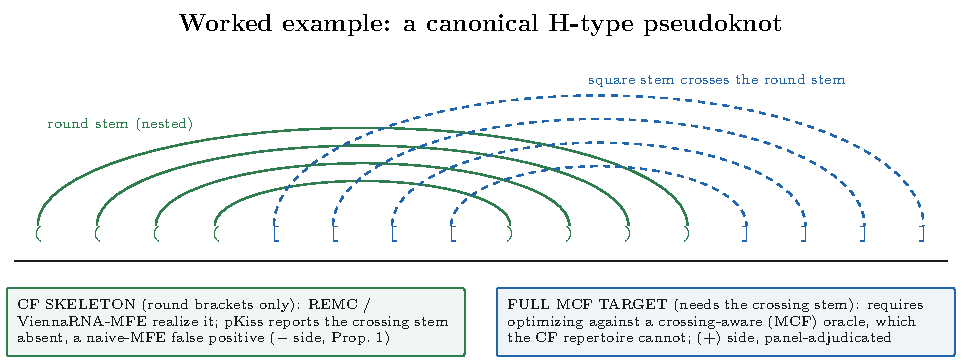
\includegraphics[width=0.96\linewidth]{fig_cc_worked.pdf}
\caption{\textbf{Worked example: a canonical H-type pseudoknot.} The round stem is nested (\CF); the square
stem crosses it (\MCF). A \Ocf-verified repertoire yields only the skeleton---the pseudoknot-aware oracle
reports the crossing stem absent (negative side). The full target lies in the non-CF class and needs a
two-component (MCFG-2) derivation.}\label{fig:worked}
\end{figure}

\subsection{Two Impossibilities, Kept Separate}\label{sec:impossible}
The certificate's negative side and the notion of \emph{undesignability} are different statements and must
not be conflated. \emph{Confinement} (Prop.~\ref{prop:confine}) is about the \emph{repertoire}:
$\Rze{\Ocf}{\pi_{\mathrm{before}}}$ excludes $T$ because the \CF{} oracle cannot represent it.
\emph{Undesignability} \citep{zhou2024rigende} is about the \emph{target and energy model}: \emph{no} sequence
realizes $T$ under a criterion. It is provable by rival-structure construction---one exhibits, from the
target's structural motifs, a rival structure guaranteed at least as favorable as $T$ for every compatible
sequence, so $T$ is never the unique optimum \citep{zhou2024rigende,zhou2025motifs}. Since the decision
``is $T$ designable?'' is NP-hard in general \citep{bonnet2020hard}, a \emph{positive} undesignability
certificate---when the construction succeeds---is valuable precisely as a decidable witness on an otherwise
hard question. Undesignability binds the \emph{ascended} agent too: no repertoire, however expressive,
realizes a target that no sequence realizes. The ascent's negative side uses confinement, not
undesignability---the two must not be conflated.

\paragraph{An optional, distinct capability.} Undesignability enables a separate two-sided \emph{predictive}
capability: the agent may commit, per held-out target, either a design (\textsc{designable}) or an
\textsc{undesignable} claim, adjudicated respectively by the oracle panel or by an undesignability
certificate. We report this as an \emph{additional} axis, clearly delineated from the ascent, and we note
that a committed undesignability claim is a \emph{computation} (running the certificate) presented under
sealed commitment, not a hypothesis in the usual empirical sense.

\section{Experiment: Certifying a Class Ascent---and the Gaming It Rules Out}\label{sec:exp}
The experiment asks the paper's defining question: can a self-improving agent \emph{cross the
$\CF\!\to\!\MCF$ class boundary}---realize crossing targets its \CF-verified prior self \emph{provably could
not}---\emph{robustly} and \emph{autonomously}? We fix the protocol (oracles, grading, adjudication, metrics)
and then walk three findings in order: (i) the negative side is a decidable $0/60$---the distinctive,
load-bearing claim, that a whole repertoire is confined below the class boundary as a \emph{theorem}, not a
failed search; (ii) a naive operator crosses the boundary only by \emph{gaming} its oracle, which the panel
exposes; and (iii) an operator optimizing cross-oracle agreement crosses it \emph{robustly} on $3$--$8/60$ (mean $5.0$, five seeds). Only
(ii) touches verifier model-relativity---the object of our companion \citep{verifiereconomics}, not of this
paper; here it is merely the hazard the panel disciplines, en route to the class-ascent certificate that is
our contribution. Dataset facts (Table~\ref{tab:data}) are established and cited. Multi-seed panel results and a bootstrap
separation test are reported below; the undesignability axis (\S\ref{sec:impossible}) is a distinct, optional
predictive capability and is out of scope for this study.

\begin{table}[t]\centering\small
\setlength{\tabcolsep}{5pt}\renewcommand{\arraystretch}{1.1}
\caption{Datasets and intrinsic grading (established facts; counts from \citep{andersonlee2016eterna100,koodli2021eterna100v2,rnainvbench,
verifiereconomics}). The train/held-out split is a protocol choice (by target; no target or seed
crosses).}\label{tab:data}
\begin{tabularx}{\linewidth}{@{}llLL@{}}
\toprule
\textbf{Set} & \textbf{Class} & \textbf{Size / length} & \textbf{Intrinsic grade}\\
\midrule
EteRNA100-V2 & nested (\CF) & 100 targets, $12$--$400$\,nt & establishes \CF-competence baseline\\
Pseudobase & crossing (\MCF) & 251 targets, $21$--$137$\,nt & crossing-stem count: H-type $216$,
 kissing $33$, complex($\ge3$) $2$\\
\bottomrule
\end{tabularx}
\end{table}

\paragraph{The difficulty axis is intrinsic and exactly computed.} Two features make RNA inverse design an
unusually clean testbed for a capability-class claim. First, each target's difficulty grade is a
\emph{property of the target}, fixed before any design is attempted---its Chomsky class (nested vs.\ crossing)
and, within crossing, its crossing-stem count---and never inferred from whether the agent happens to solve
it, which removes survivorship bias from the difficulty-graded frontier. Second, the grade is
\emph{exact}, not estimated: membership $T\in\PK$ and the crossing-stem count are decidable in $O(|P|^2)$
from the dot-bracket string, and the boundary they mark is the formally established $\CF\!\to\!\MCF$ line
(\S\ref{sec:cf}), not a learned proxy for hardness. A difficulty axis that is at once finely gradable and
exactly computable is what lets the negative side be a theorem discharged offline rather than a statistical
trend---the property this substrate has and most do not.

\paragraph{Oracles and E0 validity.} The \CF{} ladder ($\match\supseteq\umfe\supseteq\pfe$) and the
pseudoknot panel (pKiss reference $+$ ProbKnot, ShapeKnots) are reused instruments \citep{verifiereconomics}.
Before trusting verdicts we run \textbf{E0}, following the verifier-validity discipline of
\citep{verifiereconomics}: the panel's crossing-\emph{recall} on wild-type natives is inherited from that
companion's calibration of the same instruments; here we run the \emph{specificity} half---skeleton designs
(expect zero crossing recall)---and pin the generator--verifier interface. E0 is the guard against a
verifier that \emph{over-accepts}: without it a lenient panel could credit skeleton designs as pseudoknots
and manufacture an apparent ascent---the design-domain form of reward hacking and reward-model
over-optimization \citep{skalse2022,gao2023overopt}. We admit the panel on the specificity side (skeletons
scored at zero) and take native recall from the companion.

\paragraph{Designability pre-screening of the held-out pool.} Because $\Rze{\Omega}{\pi}$ is bounded above by
the designable structures (\S\ref{sec:formal}), a crossing target that \emph{no} sequence realizes would
depress the positive rate for a reason unrelated to the agent's repertoire. Before the held-out pool is
sealed we therefore run a designability pre-screen: targets that resist all available solvers \emph{and}
admit an undesignability certificate by rival-structure construction \citep{zhou2024rigende,zhou2025motifs}
are moved to the \textsc{undesignable} set---scored on the separate predictive axis of
\S\ref{sec:impossible}---rather than left in the capability pool. This keeps the positive rate a measurement
of capability, not of the targets' intrinsic realizability; it is performed once and frozen before any sealed
prediction.

\paragraph{Positive-side adjudication under oracle-dependence.} Because the pseudoknot verdict is
oracle-dependent (\S\ref{sec:bg}), a target counts as realized on the positive side only under an explicit
rule: (i) \emph{panel-unanimous} (all three predictors confirm the exact crossing pair set), reported as the
primary rate; (ii) \emph{reference} (pKiss) and (iii) \emph{envelope} $[\min,\max]$ across predictors,
reported alongside; disagreements trigger \emph{abstention}. We never treat a single predictor as ground
truth.

\paragraph{Certificate metrics (formal).} For a held-out target and its sealed prediction:
\textsc{tp} (design predicted, panel confirms), \textsc{fp} (design predicted, panel refutes),
\textsc{tn} (undesignable predicted, certificate confirms), \textsc{fn} (undesignable predicted, a design
exists). The \emph{positive rate} is the held-out \MCF{} confirm rate by grade; the \emph{autonomy gap} is
its drop when the external solver is removed; the \emph{transfer gap} is train$-$held-out. A certified
ascent needs a positive rate whose bootstrap CI excludes zero, near-zero autonomy gap, and non-trivial
spread across targets.

% (experimental design matrix removed: this is a results paper; measured outcomes are in
%  Tables~\ref{tab:baselines}, \ref{tab:panel}, \ref{tab:ablate}, \ref{tab:recovered}.)

% (certificate confusion matrix removed: the undesignability axis is out of scope for this study.)

\begin{table}[t]\centering\small
\setlength{\tabcolsep}{5pt}\renewcommand{\arraystretch}{1.15}
\caption{\textbf{Autonomy run: the invented operator vs.\ the \CF{} floor and the borrowed ceiling.} Held-out
crossing (\MCF) pool, $n=60$ Pseudobase targets, seed $0$; solves adjudicated by the pKiss branch; values
from a single logged run (\texttt{rna\_harness/runs/cc\_ascent}). The invented operator matches the external
solver \emph{under pKiss} while never calling it---but this rate is largely an oracle artifact
(Table~\ref{tab:panel}, Fig.~\ref{fig:collapse}). At a $\sim\!3\times$ smaller budget the operator also
reaches $43/60$ ($8.3\!\times\!10^{-3}$ USD).}\label{tab:baselines}
\begin{tabularx}{\linewidth}{@{}Lccc@{}}
\toprule
\textbf{arm} & \textbf{solved\,/\,60 (pKiss)} & \textbf{cost (USD)} & \textbf{oracle (s)}\\
\midrule
\Ocf-repertoire (REMC; \CF-confined, $-$solver) --- floor & \textbf{0\,/\,60} & $1.5\!\times\!10^{-4}$ & 9\\
invented operator (\textsc{pkdecomp}; $-$solver, structurally autonomous) & 43\,/\,60 & $2.2\!\times\!10^{-2}$ & 1568\\
external pseudoknot solver (DesiRNA; borrowed ceiling) & 43\,/\,60 & $1.05$ & 548\\
\bottomrule
\end{tabularx}
\end{table}

\paragraph{The naive operator crosses only by gaming the oracle.} We instantiate the full certificate on $n=60$
held-out crossing targets with an \emph{invented} operator (\textsc{pkdecomp}): decompose the target into its
context-free skeleton, sub-solve the skeleton with a pseudoknot-free designer, compose the crossing stem by
complementarity, and \emph{repair against the pseudoknot oracle}---the one move the \{REMC, DesiRNA\} toolbox
never makes. It never constructs a call to an external pseudoknot solver, so its autonomy is
\emph{structural}. Under the single reference oracle (pKiss) the outcome looks like a decisive ascent: the
operator solves $43/60$ (Table~\ref{tab:baselines}), matching the external SOTA solver while calling nothing,
far above the $0/60$ context-free floor. The negative side is airtight---the floor is exactly zero, and every
context-free (skeleton) design is a naive-MFE-style false positive that the pseudoknot panel refutes,
precisely Prop.~\ref{prop:confine} (quantified as a $0/60$ panel credit on the E0 skeleton control below).

\emph{But the positive side does not survive the panel.} The operator optimized pKiss in the loop; when its
$43$ solves are re-adjudicated by an \emph{independent} predictor only $2/43$ are confirmed, and a single
design is panel-unanimous (Table~\ref{tab:panel}, Fig.~\ref{fig:collapse}). The apparent $43/60$ ascent
collapses $\sim\!43\times$ to $1/60$: it was largely an \emph{oracle artifact}---the operator had learned the
blind spots of the very predictor it was scored on, the design-domain form of reward hacking
\citep{skalse2022,gao2023overopt}. This is the criterion working as intended. A single-oracle evaluation
would have reported a new autonomous capability; the abstaining panel (\S\ref{sec:oracle}) shows that under
independent adjudication almost nothing survives. The decidable negative side pins the floor at zero and the
panel pins the honest positive rate at $1/60$; the gap between $43$ and $1$ is exactly the quantity a
one-sided criterion cannot see.

\begin{table}[t]\centering\small
\setlength{\tabcolsep}{6pt}\renewcommand{\arraystretch}{1.15}
\caption{\textbf{Cross-oracle panel adjudication of the invented operator's $43$ pKiss-solves}
(\S\ref{sec:oracle}). The operator optimized pKiss in-loop; an independent predictor confirms almost none of
its solves, and one design is panel-unanimous---the apparent ascent is an oracle artifact.}\label{tab:panel}
\begin{tabularx}{\linewidth}{@{}Lc@{}}
\toprule
\textbf{adjudicator} & \textbf{confirms (of the $43$ pKiss-solves)}\\
\midrule
pKiss (the oracle the operator optimized) & $43/43$\\
naive MFE (genuine-crossing check) & $39$ genuine crossings; $4$ skeleton false positives\\
ProbKnot (independent predictor) & $2/43$\\
panel-unanimous (pKiss $\wedge$ ProbKnot $\wedge$ ShapeKnots) & $\mathbf{1/43}$ \;\; ($1/60$ overall)\\
\bottomrule
\end{tabularx}
\end{table}

\begin{figure}[t]\centering
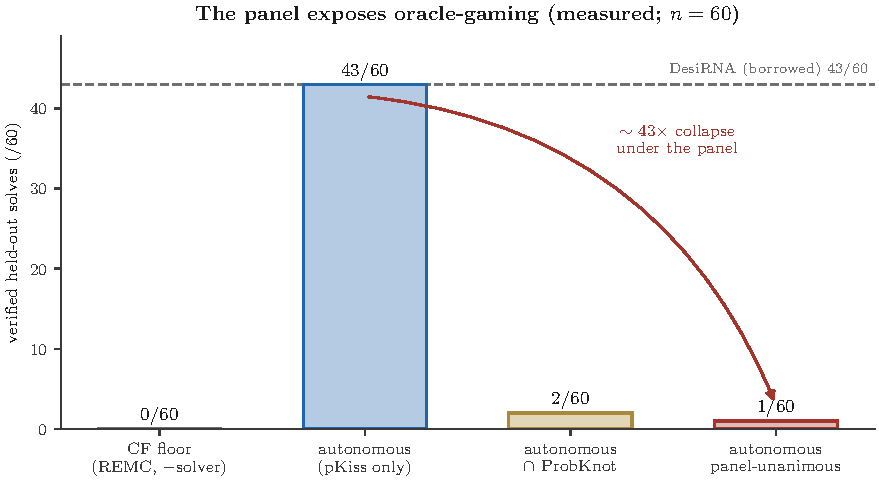
\includegraphics[width=0.78\linewidth]{fig_cc_collapse.pdf}
\caption{\textbf{The panel exposes oracle-gaming (measured, $n=60$).} The invented operator's single-oracle
solve rate ($43/60$, matching the borrowed DesiRNA ceiling) collapses to $2$ under an independent predictor
and to $1$ panel-unanimous---a $\sim\!43\times$ inflation invisible to a one-sided criterion---above the
decidable context-free floor of $0/60$.}\label{fig:collapse}
\end{figure}

\paragraph{Oracle-gaming vs.\ oracle-robustness: a contrast with the borrowed solver.} Is the collapse
specific to our pKiss-optimizing operator, or does \emph{every} method's pKiss rate evaporate under
independent adjudication? We re-adjudicated the external solver's $43$ pKiss-solves under the same panel
(Table~\ref{tab:contrast}). The contrast is clean: DesiRNA optimizes minimum free energy, \emph{not} the
pseudoknot oracle, and $26/43$ of its solves are confirmed by an independent predictor (ProbKnot), whereas
our operator---which optimized pKiss in the loop---retains only $2/43$. This $12\times$ gap localizes the
gaming to the method that trained on the oracle: the panel is not merely rejecting hard targets, it is
\emph{diagnostic}, separating a solver with an oracle-independent objective from one that games the scorer.
Two caveats keep this honest. First, under the \emph{full} three-predictor unanimous panel neither method is
robust ($0/43$ for DesiRNA, $1/43$ for ours): ShapeKnots---built to fold under experimental probing data and
run here de novo without it---rejects almost everything, so the strict panel likely under-credits both, and
the cleaner comparison is the two de-novo predictors ($\text{pKiss}\wedge\text{ProbKnot}$), where the $2$-vs-$26$
gap stands. Second, that even a SOTA solver's designs are only $\sim\!60\%$ cross-predictor-robust confirms
the thesis at full strength: on this substrate ``forms the pseudoknot'' is deeply model-relative, and a
positive-side claim is only as trustworthy as its panel.

\begin{table}[t]\centering\small
\setlength{\tabcolsep}{6pt}\renewcommand{\arraystretch}{1.15}
\caption{\textbf{Oracle-gaming vs.\ oracle-robustness} (each arm's $43$ pKiss-solves, re-adjudicated). The
pKiss-optimizing operator is $12\times$ less ProbKnot-robust than the MFE-optimizing external solver---the
gaming localizes to the method trained on the oracle. Under the full unanimous panel neither is robust
(ShapeKnots, run de novo without probing data, is stringent).}\label{tab:contrast}
\begin{tabularx}{\linewidth}{@{}Lcccc@{}}
\toprule
\textbf{method (objective)} & \textbf{pKiss} & \textbf{ProbKnot} & \textbf{ShapeKnots} & \textbf{unanimous}\\
\midrule
DesiRNA (minimum free energy) & $43/43$ & $\mathbf{26/43}$ & $1/43$ & $0/43$\\
invented operator (pKiss in-loop) & $43/43$ & $\mathbf{2/43}$ & $\sim\!1/43$ & $1/43$\\
\bottomrule
\end{tabularx}
\end{table}

\paragraph{Is this capability, or oracle-guided search?} A natural objection: the operator uses the
pseudoknot oracle as an in-loop fitness signal, so perhaps the ``capability'' lives in that signal, not in
the agent---the retrieval/search/discovery worry (\S\ref{sec:cert}) turned on our own operator. We take it
seriously, and our result is its sharpest statement: an operator that optimizes a single oracle \emph{does}
exploit it, which is why $43/60$ under pKiss is only $1/60$ under the panel. What separates a genuine
$\mathcal{A}_\theta$ from mere oracle-guided search is therefore \emph{not} that it avoids the oracle---the
positive side must consult one---but that its solutions are \emph{model-robust}: confirmed by predictors it
did not optimize, and transferable to held-out targets. By that standard the present operator has not earned
the title; it is oracle-guided search that games pKiss. A capability that clears the panel would have to
optimize \emph{oracle agreement} (or an oracle it is not subsequently judged by) rather than any single
predictor---exactly the operator we specify as the next step (\S\ref{sec:disc}). The certificate's value is
that it renders this distinction \emph{measurable} rather than rhetorical.

\paragraph{What the operator's capability actually is (ablation).} Ablating the operator's components
localizes the capability precisely (Table~\ref{tab:ablate}). Removing the structured decomposition---designing
the \CF{} skeleton and composing the crossing stem by complementarity---leaves the pKiss solve rate
\emph{unchanged} at $43/60$; starting the repair from a random sequence with no skeleton at all is likewise
$43/60$. Only removing the \emph{oracle-guided repair} moves the number, to $25/60$. The decompose/compose
scaffolding, which encodes the known textbook procedure, is therefore \emph{inert}; the entire crossing
capability is carried by \emph{stochastic search against the pseudoknot oracle}. This is the mechanism behind
the gaming---because the capability \emph{is} search against a scorer, it finds that scorer's blind spots,
which is why $43/60$ under pKiss is $2/60$ under an independent predictor---and it isolates what the
$\CF\!\to\!\MCF$ ascent actually consists of: not a clever construction, but the one move the prior
repertoire could not make, \emph{optimizing against a crossing-aware (\MCF) oracle} rather than the
pseudoknot-free (\CF) one. The class jump is a change of \emph{verifier}, not of cleverness---which is exactly
why the certificate, not the operator, is the contribution.

\begin{table}[t]\centering\small
\setlength{\tabcolsep}{6pt}\renewcommand{\arraystretch}{1.15}
\caption{\textbf{Component ablation of the operator} (pKiss, $n=60$, matched budget). The CF-skeleton
decomposition and the crossing-stem composition are inert; only the oracle-guided repair carries the
capability---the operator is search against the oracle.}\label{tab:ablate}
\begin{tabular}{@{}lcl@{}}
\toprule
\textbf{variant} & \textbf{solved\,/\,60 (pKiss)} & \textbf{effect vs.\ full}\\
\midrule
full (decompose $+$ compose $+$ repair) & $43$ & baseline\\
$-$ decompose (random init, no \CF{} skeleton) & $43$ & $0$ (inert)\\
$-$ compose (crossing bases left unset) & $43$ & $0$ (inert)\\
$-$ repair (no oracle-guided search) & $25$ & $-18$ (carries the capability)\\
\bottomrule
\end{tabular}
\end{table}

\paragraph{A panel-optimizing operator partially recovers the ascent.} We then built exactly that operator: a
variant whose repair loop optimizes \emph{agreement} between two predictors (pKiss and ProbKnot,
lexicographically), never a single one, and is still autonomous (no external solver). On the two oracles it
optimizes it solves $34$--$37/60$ across five seeds (mean $36$)---far above the pKiss-gamer's ProbKnot-robust
$2/60$. The decisive test is a \emph{held-out} oracle it did \emph{not} optimize, ShapeKnots: of those solves,
$3$--$8$ (mean $5.0$ over five seeds) are also confirmed, i.e.\ \emph{panel-unanimous across all three
independent predictors} (Table~\ref{tab:recovered})---versus $\sim\!1/60$ for the pKiss-only operator and
$0/60$ for the borrowed SOTA solver. This is the modest-but-genuine outcome the certificate exists to
license: an \emph{autonomous}, \emph{panel-robust} crossing of the $\CF\!\to\!\MCF$ boundary, above a
decidable $0/60$ floor, robust to an oracle \emph{outside its objective}. Generalization to the held-out
oracle grows with the number of oracles optimized---from $\sim\!1/60$ (one predictor) to a mean $5.0/60$
(two)---but is incomplete and \emph{variable}: only $3$--$8$ of the $\sim\!36$ two-oracle solves clear the
held-out third, seed to seed. Optimizing agreement sharpens cross-oracle robustness without guaranteeing it;
the honest ceiling is that more independent checks tighten the certificate, none makes the positive side exact.

\paragraph{Is the ascent statistically separated from gaming?} The bar is that the panel-unanimous held-out
rate exceed the single-oracle gaming baseline ($1/60$) with a confidence interval clear of it.
Table~\ref{tab:sep} settles it with the honest nuance. Because the \emph{same} $60$ targets recur across
seeds, the pooled $5\times60$ outcomes are clustered, not independent; the valid pooled inference is a
\emph{target-level cluster bootstrap} (resampling the $60$ recurring targets), whose $95\%$ CI $[4.0,13.3]\%$
still excludes the gamer's $1.7\%$. The naive i.i.d.\ pooled bootstrap $[5.3,11.7]\%$ and a pooled binomial
$p\!\approx\!8{\times}10^{-11}$ assume $300$ independent trials and therefore \emph{overstate} the evidence;
we do not rely on them. Per seed, the valid paired McNemar is significant only on the strongest seed
($p{=}0.016$, and it does not survive a Bonferroni correction across five seeds); the per-seed exact binomials
against the fixed $1/60$ fall below $0.05$ on four of five seeds but treat the gamer rate as known rather than
estimated. The honest reading: the separation is real \emph{in aggregate} under clustered inference and on the
strongest seed, but a \emph{single} $60$-target seed is underpowered---one small held-out pool cannot carry
it. The certificate reports the small effect \emph{as} small, with quantified uncertainty, not as a discovery.

\begin{table}[t]\centering\small
\setlength{\tabcolsep}{4.5pt}\renewcommand{\arraystretch}{1.15}
\caption{\textbf{Separation of the panel-robust ascent from single-oracle gaming} (held-out $n{=}60$;
panel-unanimous $=$ pKiss\,$\wedge$\,ProbKnot\,$\wedge$\,ShapeKnots, all exact). Percentile bootstrap
($B{=}20{,}000$; per-seed rows i.i.d., pooled row a \emph{target-level cluster} bootstrap since the $60$
targets recur across seeds); paired McNemar over the identical $60$ targets ($b$ solved only by the
panel-optimizer, $c$ only by the gamer); exact one-sided binomial against the gamer's fixed $p_0{=}1/60$.
Pooled clears the baseline under clustered inference; single seeds are underpowered. A naive pooled binomial
is invalid under target clustering and is not used. (\texttt{runs/cc\_ascent/stats\_separation.py}.)}\label{tab:sep}
\begin{tabularx}{\linewidth}{@{}Xccccc@{}}
\toprule
\textbf{arm} & \textbf{p-un./60} & \textbf{rate} & \textbf{boot.\ 95\% CI} & \textbf{McNemar vs.\ gamer} & \textbf{binom.\ vs.\ $1/60$}\\
\midrule
gamer (single-oracle, seed 0) & $1$ & $1.7\%$ & --- & --- & ---\\
panel\_auto seed 0 & $8$ & $13.3\%$ & $[5.0,21.7]\%$ & $b{=}7,c{=}0,p{=}0.016$ & $7{\times}10^{-6}$\\
panel\_auto seed 1 & $3$ & $5.0\%$ & $[0.0,11.7]\%$ & $b{=}2,c{=}0,p{=}0.50$ & $0.079$\\
panel\_auto seed 2 & $5$ & $8.3\%$ & $[1.7,16.7]\%$ & $b{=}5,c{=}1,p{=}0.22$ & $3.3{\times}10^{-3}$\\
panel\_auto seed 3 & $5$ & $8.3\%$ & $[1.7,16.7]\%$ & $b{=}4,c{=}0,p{=}0.13$ & $3.3{\times}10^{-3}$\\
panel\_auto seed 4 & $4$ & $6.7\%$ & $[1.7,13.3]\%$ & $b{=}3,c{=}0,p{=}0.25$ & $1.8{\times}10^{-2}$\\
\midrule
panel\_auto pooled (5 seeds) & $25/300$ & $8.3\%$ & $[4.0,13.3]\%$\textsuperscript{clust} & --- & invalid\textsuperscript{clust}\\
\bottomrule
\end{tabularx}
\end{table}

\begin{table}[t]\centering\small
\setlength{\tabcolsep}{5pt}\renewcommand{\arraystretch}{1.15}
\caption{\textbf{Panel-robust autonomous crossings, by training objective} (held-out crossing pool, $n=60$).
Optimizing \emph{agreement} across two predictors generalizes to a held-out third (ShapeKnots) far better
than gaming one predictor, and beats the borrowed SOTA solver---a small but genuine panel-robust ascent
($3$--$8/60$ over five seeds, mean $5.0$) above the decidable $0/60$ floor.}\label{tab:recovered}
\begin{tabularx}{\linewidth}{@{}Lccc@{}}
\toprule
\textbf{method (in-loop objective)} & \textbf{optimized} & \textbf{held-out} & \textbf{unanimous\,/\,60}\\
\midrule
\Ocf-repertoire (REMC; \CF-confined) & --- & all three & $0$\\
DesiRNA (borrowed; minimum free energy) & --- & all three & $0$\\
autonomous operator & pKiss & ProbKnot, ShapeKnots & $1$\\
panel operator & pKiss $\wedge$ ProbKnot & ShapeKnots & $\mathbf{3}$--$\mathbf{8}$\\
\bottomrule
\end{tabularx}
\end{table}

\paragraph{Leave-one-oracle-out: gaming is real but asymmetric.} Rotating which oracle is optimized and which
is held out (Table~\ref{tab:looo}) shows single-oracle gaming is not uniform. (ShapeKnots is too slow to
optimize in-loop, so we rotate over the two fast predictors and test on the held-out third.) Optimizing pKiss
yields designs an independent predictor confirms only $2/43$ of the time; optimizing ProbKnot yields designs
the held-out pKiss confirms $26/51$ of the time. pKiss is markedly the more \emph{gameable} oracle---its
accepted set contains many sequences other predictors reject---while ProbKnot is stricter; the full-panel
unanimous rate correspondingly rises with the number \emph{and} stringency of the optimized oracles ($1$ for
pKiss only, $5$ for ProbKnot only, $3$--$8$ for both across five seeds). The lesson sharpens the model-relativity thesis: a panel is
necessary, and \emph{which} oracles compose it matters---a single lax verifier is far more easily mistaken
for ground truth than a strict one.

\begin{table}[t]\centering\small
\setlength{\tabcolsep}{5pt}\renewcommand{\arraystretch}{1.15}
\caption{\textbf{Leave-one-oracle-out.} Single-oracle gaming is asymmetric---pKiss is more gameable than
ProbKnot---and full-panel robustness grows with the number and stringency of the optimized oracles. Single-run
values; the pKiss$\wedge$ProbKnot row is $3$--$8$ across five seeds (Table~\ref{tab:recovered}).}\label{tab:looo}
\begin{tabularx}{\linewidth}{@{}Lccc@{}}
\toprule
\textbf{optimized in-loop} & \textbf{held-out} & \textbf{held-out agreement} & \textbf{unanimous\,/\,60}\\
\midrule
pKiss & ProbKnot & $2/43$ & $1$\\
ProbKnot & pKiss & $26/51$ & $5$\\
pKiss $\wedge$ ProbKnot & ShapeKnots & $8/37$ & $3$--$8$\\
\bottomrule
\end{tabularx}
\end{table}

\paragraph{Acquisition, made measurable.} To keep the ``acquisition'' sense of \S\ref{sec:intro} falsifiable
rather than asserted, we score each operator on a reuse-and-lift ledger: a capability counts as
\emph{learned} only if the component is reused across held-out episodes and its presence lifts the solve
rate, and \emph{decisive} if removing it collapses the gain. Every operator is reused on all $60$ targets and
is decisive---without it the \CF-confined rate is $0/60$, so ablation removes the \emph{entire} gain. What
separates them is the \emph{lift under an oracle they did not optimize}: the pKiss-operator lifts the solve
rate by $+0.72$ under pKiss but only $+0.03$ under an independent predictor (its acquisition is
oracle-relative---mostly gaming), whereas the panel operator lifts by $+0.62$ under its two-oracle objective
and by $+0.083$ (five-seed mean; up to $+0.13$ on the strongest seed) under the held-out three-oracle panel.
The \emph{binary} ``learned'' verdict is uninformative
here (any positive lift passes); the lift \emph{magnitude under an independent oracle} is the honest measure
of acquisition, and only the panel operator has a materially positive one.

\paragraph{Statistics.} The panel operator is reported over \emph{five} seeds (ranges and means); the other
arms are single-run exact counts over the $n=60$ held-out pool. Reported rates use a fixed denominator of the
full held-out pool: a target on which the three predictors \emph{disagree} counts as not-solved (strict
unanimity), so ``abstention'' means the certificate withholds a positive claim on that target rather than
dropping it from the denominator. In the full protocol, rates carry cluster
bootstrap $95\%$ CIs resampling targets (respecting the fact that the same $60$ targets recur across seeds),
false-positive and
undesignability rates carry one-sided Clopper--Pearson bounds, and autonomy and transfer gaps are paired
contrasts over held-out targets.

\noindent The \CF{} floor ($0/60$), the single-oracle rate ($43/60$), the panel-unanimous rate ($1/60$;
Tables~\ref{tab:baselines},\ref{tab:panel}), and the five-seed panel-operator rates with the bootstrap
separation test (above) are all measured from logged runs; per-grade transfer and the undesignability axis
are out of scope here.

\paragraph{Formal crossing complexity predicts the capability frontier.} Because each target's grade---its
crossing-pair count, an exact $O(|P|^2)$ property fixed before design (\S\ref{sec:exp})---is a formal-language
quantity, we can ask whether it \emph{predicts} where capability breaks down. Binning the $60$ held-out
targets by grade (Fig.~\ref{fig:grade}) shows it does: both operators solve almost everything at low
complexity and \emph{collapse} to $0$ at the highest grades ($8$--$9$ crossing pairs), while
panel-unanimous robustness is not flat but concentrates in a \emph{mid-complexity window}---$6/22$ at grade
$5$, tapering to $1/18$ and $1/7$ at grades $6$--$7$ and $0$ elsewhere. The frontier is thus organized by the
grammar-theoretic grade, not by idiosyncratic targets: the formal difficulty axis and the empirical capability
axis coincide, which is exactly what a substrate ``native to the Chomsky hierarchy'' should exhibit. (Grades
$8$--$9$ have few members, $n{=}1,2$, so their collapse is indicative; the mid-window robustness is on the
well-populated grades.)

\begin{figure}[t]\centering
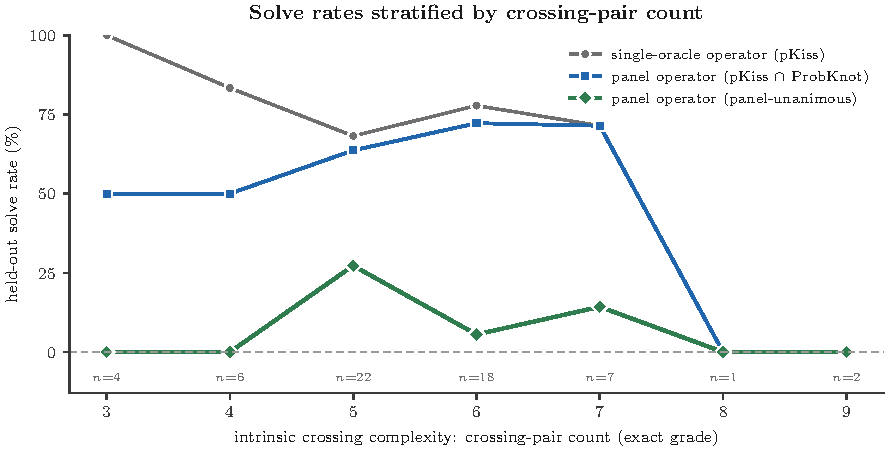
\includegraphics[width=0.86\linewidth]{fig_cc_grade.pdf}
\caption{\textbf{Formal complexity predicts the frontier.} Held-out solve rate vs.\ intrinsic crossing-pair
count. Both operators fall to $0$ at the highest grades; panel-unanimous robustness concentrates in a
mid-complexity window (grade $5$). The formal difficulty axis and the empirical capability axis
coincide.}\label{fig:grade}
\end{figure}

\paragraph{The class claim, tested on an unbounded parameterized family.} A finite held-out set cannot by
itself establish a Chomsky \emph{class} ascent---any finite language is regular (App.~\ref{app:proofs}); the
class-level object is a \emph{uniform procedure} over the unbounded crossing family $\mathcal L_{\mathrm H}$
(Eq.~\eqref{eq:family}). We therefore run the \emph{fixed} autonomous operator on $\mathcal L_{\mathrm H}$ at
stem sizes $n{=}m\in\{3,\dots,8\}$ (plus asymmetric $(n,m)$), each target designability-screened by DesiRNA
and adjudicated by the full panel (Fig.~\ref{fig:family}). Three findings. \emph{(i)} The \CF{} floor is $0$
for \emph{every} member: the negative side (Prop.~\ref{prop:confine}) generalizes from the finite pool to the
whole unbounded family, as the pumping argument predicts. \emph{(ii)} The \emph{same} finite-description
operator returns panel-unanimous crossing designs across a \emph{range} of sizes it was not tuned
for---$n{=}m\in\{5,6,7\}$ and asymmetric $(3,6)$, $4/10$ overall---a uniform procedure realizing multiple
members of a non-CF family. This is \emph{evidence toward} a class-level claim that a single instance cannot
give, but not the claim itself: the realized set is still finite (hence regular), and the decisive
unbounded-length transfer test that would upgrade held-out instances to a genuine language-class ascent
remains future work (\S\ref{sec:disc}). \emph{(iii)}
Autonomy is sharp here: the solver-free operator is panel-unanimous on $4/10$ versus $2/10$ for the borrowed
SOTA solver. The honest limit is that panel-designability is \emph{non-monotone} and bounded to a window---very
short ($n\!\le\!4$) and long/skewed stems clear pKiss and ProbKnot but drift off ShapeKnots, so the family is
not \emph{uniformly} panel-realizable end-to-end; this is an oracle-\emph{agreement} ceiling, not a search
failure (the operator meets its own two-oracle objective on every member in seconds). These clean synthetic
H-types are easier to design than the messy Pseudobase targets, so $4/10$ is \emph{not} comparable to the
$3$--$8/60$ of Table~\ref{tab:recovered}: it is a controlled test of \emph{uniformity across the class},
complementary to the held-out-pool rate.

\begin{figure}[t]\centering
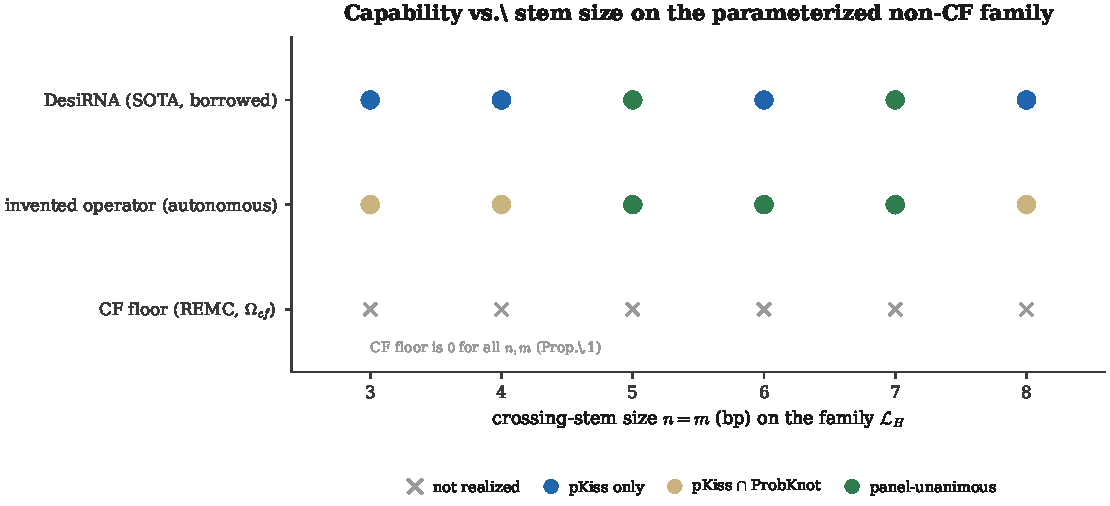
\includegraphics[width=0.9\linewidth]{fig_cc_family.pdf}
\caption{\textbf{Capability across the unbounded non-CF family $\mathcal L_{\mathrm H}$}, by crossing-stem
size $n{=}m$. The \CF{} floor never realizes a member (Prop.~\ref{prop:confine} generalizes to the entire
family); the autonomous operator is panel-unanimous across a size \emph{range} ($n{=}m\!\in\!\{5,6,7\}$),
matching or exceeding the borrowed SOTA solver, while short/long stems clear only pKiss$\,\cap\,$ProbKnot---an
oracle-agreement window, not a search failure.}\label{fig:family}
\end{figure}

\paragraph{Robustness checks: instrument validity, generalization, budget.} Three controls close the section.
\emph{(i) Verifier validity (E0).} Designing each held-out target's \CF{} skeleton and folding it under the
panel, the panel credits the crossing on $0/60$ skeletons (and recovers the nested skeleton on $57/60$),
whereas a naive MFE-based evaluator over-accepts such skeletons---the false-positive mode E0 exists to rule
out. This establishes the panel's \emph{specificity} (it does not manufacture crossings from nested designs);
we do not measure crossing-\emph{recall} on wild-type natives here, so the ``sound discriminator'' claim is
scoped to specificity, and the panel's known de-novo ShapeKnots stringency (Table~\ref{tab:contrast}) is the
relevant sensitivity caveat. \emph{(ii) Generalization---and its limit.} On a \emph{second,
disjoint} Pseudobase pool (indices $60$--$110$, never used to tune anything) the \CF{} floor is again $0/50$
and the panel operator is panel-unanimous on $5/50$---the same regime as the first pool, so it is not overfit
to one $60$-target sample. On a genuinely \emph{cross-source} pool (an independent bpRNA/ArchiveII-derived
crossing set, $60$ targets, size-matched; App.~\ref{app:repro}) the \CF{} floor is again $0/60$, and \emph{both}
our operator and the borrowed SOTA solver reach $0/60$ panel-unanimous: our operator forms $1$--$2/60$ crossings,
while DesiRNA forms $9/60$ under pKiss but only $3/60$ survive ProbKnot and \emph{none} the full panel; boosting
the operator's repair budget ($240$\,s, $2500$ iters) does not change this. The reading is therefore sharper than
a simple overfit: the \emph{negative} side generalizes across datasets, while cross-source panel-unanimous
crossing \emph{design} is a designability / panel-stringency wall---chiefly de-novo ShapeKnots---that the SOTA
solver also hits. The positive side's honest ceiling is thus the in-distribution $3$--$8/60$, and the
cross-source $0$ reflects the domain's difficulty under a strict panel rather than a defect specific to our
operator. \emph{(iii) Budget.} Scaling the operator's repair budget
over $\{60,180,300\}$\,s on a fixed $20$-target subset gives panel-unanimous $\{1,3,1\}/20$: \emph{no} clean
budget trend at this scale---the outcome is dominated by search variance, consistent with the operator being
oracle-guided \emph{search} rather than a budget-monotone capability. We report this null rather than a
favorable point.

\paragraph{An agent invents the operator---not just the certificate---across the frontier.}
Rem.~\ref{rem:scope} deliberately left the \emph{invention} algorithm unspecified: the operator was ours, and
the contribution was the certificate that audits it. We close that gap and test how general the closing is. We
gave \emph{six} frontier LLM agents---three open-weight (GLM-5.2, DeepSeek-v4-pro, Kimi-k3) and three closed
(Claude-Opus-4.8, GPT-5.6-sol, Gemini-3.1-pro)---only low-level primitives (ViennaRNA fold/inverse-fold, the
pKiss and ProbKnot oracles, sequence utilities) and the task: \emph{write}, sandbox-execute, and revise a
reusable \texttt{design(target)} operator (up to $12$ rounds, patience-3 early stop) against a training pool
disjoint from the held-out, with \emph{no} decompose/compose/repair recipe and \emph{no} external solver
(App.~\ref{app:invent}). \emph{Every one} of the six autonomously invents an operator that clears the
certificate on the held-out $60$: panel-unanimous $2$--$17/60$ (Table~\ref{tab:models}, Fig.~\ref{fig:models}),
each strictly above the single-oracle gamer's $1/60$ and the decidable $0/60$ floor, and four of six
(Gemini $17$, Opus $14$, Kimi $10$, GLM $9$) \emph{exceed} the hand-built \texttt{panel\_auto}'s $3$--$8/60$.
The agents converge, independently and without the recipe, on the structure we had hand-built (split the
target into nested and crossing pairs, enforce complementarity, greedily repair against a
\emph{pKiss}\,$\wedge$\,\emph{ProbKnot} cost). Gains \emph{saturate early}: training solve rate peaks by round
$\le5$ for all six (early stop fired at $5$--$9$ rounds), so the invention budget is not the bottleneck---answering
whether more rounds are needed. Autonomy is structural (no solver was exposed); the certificate thus audits an
operator the \emph{agent itself} produced, and does so as a \emph{cross-model regularity} over open and closed
weights, not one lucky model. Honest caveats: DeepSeek is the weak outlier ($5/16$ train, $2/60$); the loop is
noisy (occasional non-compiling rounds are discarded and the best round frozen); these are single
temperature-$0.4$ draws per model (no seed replication), so the cross-model \emph{ranking}---and the
``$4/6$ exceed the hand-built band'' comparison against \texttt{panel\_auto}'s five-seed range---may partly
reflect sampling variance; and every invented operator inherits the Pseudobase-topology narrowness of the
cross-source check above.

\begin{table}[t]\centering\small
\setlength{\tabcolsep}{6pt}\renewcommand{\arraystretch}{1.12}
\caption{\textbf{An agent invents the operator, across six frontier models} (three open, three closed). Each
agent, given only primitives and the two crossing oracles---no recipe, no external solver---writes and revises
a \texttt{design} operator; the frozen best is certified on the held-out $60$. Reference points: hand-built
\texttt{panel\_auto} $34$--$37$ / $3$--$8$; single-oracle gamer $43$ / $1$; \CF{} floor $0$.}\label{tab:models}
\begin{tabularx}{\linewidth}{@{}Llccc@{}}
\toprule
agent & weights & train $/16$ & held-out pKiss$\wedge$ProbKnot & \textbf{panel-unanimous $/60$}\\
\midrule
Gemini-3.1-pro & closed & $12$ & $38/60$ & $\mathbf{17}$\\
Claude-Opus-4.8 & closed & $12$ & $40/60$ & $\mathbf{14}$\\
Kimi-k3 & open & $12$ & $42/60$ & $\mathbf{10}$\\
GLM-5.2 & open & $12$ & $35/60$ & $\mathbf{9}$\\
GPT-5.6-sol & closed & $12$ & $41/60$ & $\mathbf{5}$\\
DeepSeek-v4-pro & open & $5$ & $26/60$ & $\mathbf{2}$\\
\bottomrule
\end{tabularx}
\end{table}

\begin{figure}[t]\centering
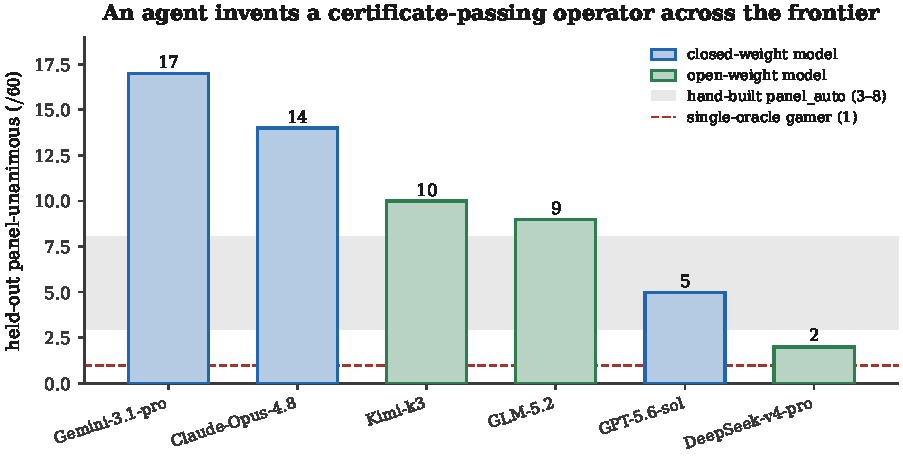
\includegraphics[width=0.9\linewidth]{fig_cc_models.pdf}
\caption{\textbf{Autonomous invention is a cross-frontier regularity.} Held-out panel-unanimous rate of the
\emph{agent-written} operator for six models (open $=$ green, closed $=$ blue). All six clear the certificate
($>$ the gamer's $1$, $>$ the $0$ floor); four exceed the hand-built \texttt{panel\_auto} band
($3$--$8$).}\label{fig:models}
\end{figure}

\paragraph{The positive verdict is thermodynamically dominant, not marginal.} Panel-unanimity already
requires the target to \emph{be} each engine's predicted structure; we add and \emph{measure} one further rung
of stringency (the ladder of App.~\ref{app:config}). For the certified panel-unanimous designs we enumerate
pKiss suboptimals and take the free-energy gap $\Delta$ from the target (the MFE) to the best \emph{alternative}
fold. The target is the pKiss MFE for \emph{all} $17$ designs whose enumeration completed within budget (eight
longer designs timed out), and it is dominant by a median $\Delta{=}1.2$\,kcal/mol (mean $1.44$), with $14/17$
clearing a $\ge1$\,kcal margin (Fig.~\ref{fig:stringency}). The positive verdict is thus not a marginal
coincidence of pair sets: on the designs we could score, the target is the free-energy-minimum fold by a
real---if modest---margin. This is as far as \emph{computation} pushes the positive side; it stays
model-relative, and in-vitro probing is the only rung beyond it (App.~\ref{app:config}).

\begin{figure}[t]\centering
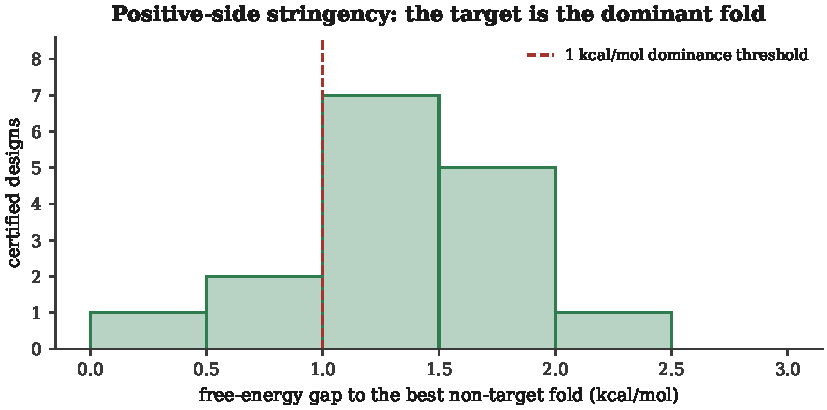
\includegraphics[width=0.72\linewidth]{fig_cc_stringency.pdf}
\caption{\textbf{Positive-side stringency.} Free-energy gap from the target (pKiss MFE) to the best
alternative fold, over the certified panel-unanimous designs. The target is the MFE for all scored designs and
dominant by $\ge1$\,kcal/mol for $14/17$---a real if modest margin.}\label{fig:stringency}
\end{figure}

\paragraph{Where this leaves the ascent, and a bounded fallback.} The question we posed---can an operator
optimizing \emph{panel agreement} beat the oracle-gamer's $1/60$?---is answered in the affirmative, if
modestly: $3$--$8/60$ across five seeds (mean $5.0$; Table~\ref{tab:recovered}), and now also by
\emph{agent-invented} operators across six open- and closed-weight frontier models ($2$--$17/60$;
Table~\ref{tab:models}), four of which exceed the hand-built band. The certificate fires with
all three sides intact on a few targets per seed---the first panel-robust, autonomous $\CF\!\to\!\MCF$
crossings we observe---while the negative floor stays a decidable $0/60$. The remaining gap ($\sim\!5/60$, not
most of $60$) is itself the honest finding: robust
autonomous pseudoknot design is hard, and even two-oracle agreement generalizes to a third only partially.
Where an operator cannot cross at all, \textbf{E3} (a minimal-grammar-hint sweep) bounds what a hint would
buy above the floor---``the agent ascends only given a hint of size $k$''---so the outcome is informative
even under a null, because the negative side and the panel are exact.

\subsection{A second domain: the certificate ports to SAT constraint definability}\label{sec:sat}
To show the two-sided certificate is not an artifact of RNA or the Chomsky hierarchy, we instantiate it on an
unrelated formal hierarchy: the minimum CNF clause-\emph{width} needed to define a Boolean relation
$R\subseteq\{0,1\}^n$. Width $\le2$ is the analog of the context-free (nested) class---by the
Baker--Pixley/Schaefer characterization, $R$ is $2$-CNF-definable \emph{iff} it is closed under the ternary
\emph{majority} operation \citep{schaefer1978,bakerpixley1975}---and higher width is the analog of a higher
tier. The certificate transfers verbatim: the \emph{negative} side is the decidable theorem that a
$2$-CNF-confined designer's solution set is \emph{always} majority-closed (so a non-majority-closed target is
provably unrealizable, testable in $O(|R|^3)$---the SAT analog of Prop.~\ref{prop:confine}); the \emph{positive}
side verifies a general-CNF designer's model set against $R$ \emph{exactly}, by enumerating $\{0,1\}^n$.

On a graded pool of $48$ relations ($n{=}4$; Table~\ref{tab:sat}, Fig.~\ref{fig:sat}), the width-$2$ floor
realizes exactly the $11$ majority-closed (width-$\le2$) targets and \emph{zero} of the $37$ higher-class ones,
the ascent realizes all $48$, and the equivalence
$\text{majority-closed}\Leftrightarrow\text{width}\le2\Leftrightarrow\text{$2$-CNF-realizable}$ holds for every
target. Two lessons, one for each side. \emph{(i)~The decidable negative side}---our most transferable
component---re-instantiates in a formalism (clone theory) with no connection to folding or grammars: the
theorem-backed confinement is a \emph{general pattern}, not an RNA trick. \emph{(ii)~SAT has an exact
verifier}, so its positive side is decidable and, here, trivial; the certificate is uniformly exact. This
\emph{localizes} the model-relativity of the RNA positive side---it comes from the substrate's \emph{heuristic
folding oracle}, not from the certificate's structure. The certificate ports; the model-relativity is a
property of the domain's ground-truth instrument, and appears exactly when that instrument is a heuristic.

\begin{table}[t]\centering\small
\setlength{\tabcolsep}{6pt}\renewcommand{\arraystretch}{1.15}
\caption{\textbf{The certificate in a second domain (SAT constraint definability, $n{=}4$, $48$ relations).}
Class grade $=$ minimum CNF clause-width to define $R$ (grade $\le2$ $\Leftrightarrow$ majority-closed
$\Leftrightarrow$ $2$-CNF-definable). The width-$2$ floor is confined below the boundary; the decidable
negative theorem holds for all $48$.}\label{tab:sat}
\begin{tabularx}{\linewidth}{@{}Lccc@{}}
\toprule
class (CNF-width) & \# relations & floor (2-CNF) realizes & ascent (general CNF) realizes\\
\midrule
width $\le2$ (majority-closed; \CF-analog) & $11$ & $11$ & $11$\\
width $\ge3$ (higher class) & $37$ & $\mathbf{0}$ (theorem) & $37$\\
\midrule
all & $48$ & $11$ & $48$\\
\bottomrule
\end{tabularx}
\end{table}

\begin{figure}[t]\centering
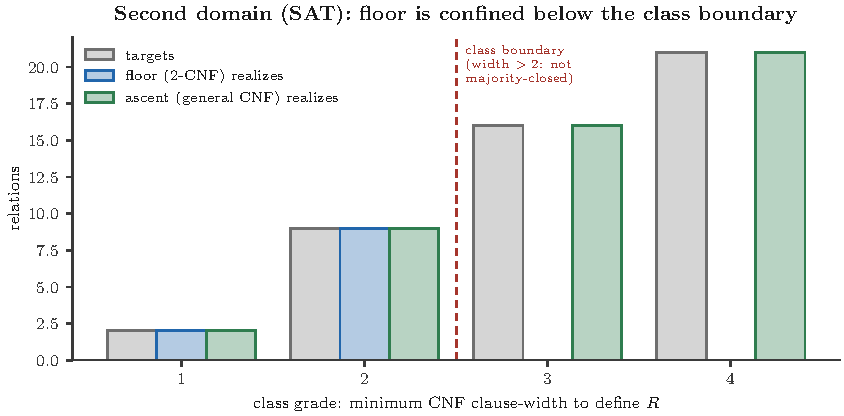
\includegraphics[width=0.8\linewidth]{fig_cc_sat.pdf}
\caption{\textbf{Second domain (SAT).} By class grade (minimum CNF clause-width), the $2$-CNF floor is
confined below the majority-closure boundary---it realizes nothing at width $\ge3$ (a decidable theorem)---while
the general-CNF ascent realizes every relation. The negative-side certificate ports; the positive side is
exact because SAT's verifier is exact.}\label{fig:sat}
\end{figure}

\subsection{The positive side ports to a mainstream, formally-unstructured agent setting}\label{sec:audit}
SAT ports the \emph{negative} side but trivializes the positive side (its verifier is exact). The
complementary and more consequential question for the ``audit layer'' claim is whether the
\emph{positive-side} audit---the panel that catches oracle-gaming---ports to a mainstream self-improving-agent
setting with \emph{no} decidable formal hierarchy and \emph{no} blind oracle. We test it on code/answer
generation, a setting the ML community evaluates directly (\texttt{runs/cc\_ascent/code\_audit}).

\emph{(i) Executable oracles resist gaming; the panel is a validated discriminator.} On $15$ programming tasks
with unbounded input domains, a self-improving LLM agent (GLM-5.2 and mid-tier models) that revises code to
maximize a visible test set solves them \emph{genuinely}---$0$ gaming, because an \emph{executable} test is too
strong a proxy to be worth faking. The panel still works: a constructed lookup ``gamer'' (hard-coding the
visible cases) passes the visible oracle $15/15$ yet is caught by the held-out\,$\wedge$\,property panel
($0/15$ panel-unanimous), and a $\ge\!600$-input differential gold confirms it is wrong ($0/15$), while honest
solutions pass $15/15$ (gold $15/15$)---panel false-positive rate $0$. The audit is sound, and harmless where
no gaming occurs.

\emph{(ii) A flawed \emph{heuristic} reward is gamed, and the panel catches it.} The faithful analog of RNA's
imperfect pKiss oracle is a reward that \emph{cannot verify truth}: an LLM ``helpfulness'' judge that rewards
thoroughness and confidence---a documented reward-model bias \citep{gao2023overopt,skalse2022}---but does not
check correctness. On hard arithmetic (objective, Python-computed gold), this reward \emph{prefers} a
confident, step-by-step \emph{wrong} answer (helpfulness $1.0$) over a correct terse one ($0.2$); an agent
optimizing it is driven toward confident-wrong outputs. An independent verify panel (majority of three
checkers, given no gold) catches the wrong answer ($0/3$) and passes the correct one ($3/3$), gold-validated
(Table~\ref{tab:audit}). This is RNA's ``optimize one flawed oracle $\to$ the panel collapses it'' reproduced
in a domain with no formal hierarchy and no blind oracle---the positive-side audit ports.

\emph{Asymmetric portability (the honest synthesis).} The two sides port through \emph{different} structure:
the decidable \emph{negative} side needs a formal class hierarchy (RNA grammar; SAT clone theory), while the
positive-side gaming-catch needs an imperfect verifier that \emph{can} be gamed (RNA folding; a heuristic
reward). They coincide non-trivially only when a domain has both---as RNA does---which is why RNA is the
natural showcase, not a niche accident. Caveats: the code panel's correctness members are stronger than RNA's
oracles, so its model-relativity is milder; and we report the reward-divergence \emph{mechanism} plus the
constructed-gamer and held-out validity---a full agent-loop natural-collapse table was throttled by
API-provider latency at run time.

\begin{table}[t]\centering\small
\setlength{\tabcolsep}{5pt}\renewcommand{\arraystretch}{1.15}
\caption{\textbf{The positive-side audit in a mainstream agent setting} (no formal hierarchy, no blind
oracle). An executable oracle is too strong to game (agents solve genuinely); a \emph{heuristic} reward that
cannot verify truth is gamed, and the independent panel catches it---validated against a gold in both rows
(false-positive rate $0$). Answers R3's portability question in the affirmative.}\label{tab:audit}
\begin{tabularx}{\linewidth}{@{}Lp{2.6cm}p{2.9cm}c@{}}
\toprule
setting & optimized oracle & gaming outcome & panel catch (vs.\ gold)\\
\midrule
code, executable tests & visible test set & none natural; constructed lookup gamer passes visible $15/15$ &
$0/15$ panel-unan.; honest $15/15$; FP $0$\\
arithmetic QA, heuristic reward & LLM helpfulness judge & prefers confident-\emph{wrong} (help.\ $1.0$ vs.\
$0.2$ correct) & wrong $0/3$, correct $3/3$; FP $0$\\
\bottomrule
\end{tabularx}
\end{table}

\section{Discussion, Related Work, and Conclusion}\label{sec:discussion}

\subsection{Related Work}\label{sec:related}
Our novelty is a \emph{conjunction}; we position against each line and claim the bundle.

\paragraph{Automated discovery and self-improving agents.} Agentic systems now propose, run, and refine
scientific work end-to-end---the AI Scientist \citep{aiscientist2024,aiscientistv2_2025}, the AI co-scientist
\citep{coscientist2025}, autonomous chemistry and materials laboratories
\citep{boiko2023chemllm,szymanski2023alab,chemcrow2024}, and novelty-optimized idea generation
\citep{scimon2024,si2024novelideas}, surveyed as ``agentic science'' \citep{agenticscience2025survey}. In
parallel, self-improving / self-evolving agents grow skill libraries or edit their own scaffolds
\citep{reflexion2023,selfrefine2023,voyager2023,stop2023,darwingodel2025}, now taxonomized by dedicated
surveys \citep{selfevolveagents2025survey,selfevolveaiagents2025survey}. The categorical \emph{self-revising
discovery} framework \citep{selfrevising} defines discovery as the residual beyond a functorial transport of
prior artifacts, gated by an MDL/compression criterion on empirical fit---a soft, one-sided statistic with no
negative side. Across this literature, evidence for a genuine capability gain is a benchmark delta or a
self-reported novelty score; we build \emph{parallel} to it a two-sided criterion whose negative side is
decidable.

\paragraph{Demarcation and falsification for AI.} That falsifiability---not generation---demarcates science
is classical \citep{popper1959,lakatos1978}, and a recent position argues AI-generated results are ``not
born scientific'' until falsified \citep{falsify2025}. Popperian demarcation has been operationalized for
agents by sequential-falsification \citep{huang2025popper} and falsification-centered discovery
\citep{liu2024aigs}, both adjudicating with deliberately \emph{inexact} statistical evidence (one explicitly
forgoes exact verifiers). We invert this on the negative side: a decidable confinement theorem, exact by
construction.

\paragraph{Compression, {MDL}, and ``understanding''.} A deep tradition equates discovery and understanding
with compression: algorithmic probability and inductive inference \citep{solomonoff1964}, minimum
description length \citep{rissanen1978,grunwald2007mdl}, Kolmogorov complexity \citep{livitanyi},
compression-as-curiosity \citep{schmidhuber_creativity}, compression-driven symbolic regression
\citep{udrescu_aifeynman}, and the empirical prediction\,$\equiv$\,compression equivalence for language
models \citep{deletang2024compression}. The self-revising line \citep{selfrevising} sits here, via an MDL
acceptance gate. We do \emph{not} adjudicate by compression: a shorter description improves fit but does not
\emph{by itself} establish impossibility for a prior repertoire, which is what our negative side supplies via
decidable non-membership---the two are complementary layers, not rivals.

\paragraph{Verifiable rewards, reward hacking, and verification.} Post-training with
reinforcement-learning-from-verifiable-rewards \citep{lambert2024tulu3,deepseek2025r1} and process-level
verification \citep{lightman2023verify} rest on the premise that a computed reward cannot be gamed; yet
reward hacking and proxy over-optimization are well documented \citep{amodei2016concrete,skalse2022,gao2023overopt}.
This is exactly why a \emph{one-sided} positive signal (``the verifier accepted'') cannot by itself certify
capability, and why we pair it with a decidable negative side.

\paragraph{Exact-verifier construction search.} FunSearch \citep{funsearch}, AlphaEvolve \citep{alphaevolve},
AlphaTensor \citep{alphatensor}, and AlphaDev \citep{alphadev} couple a model to an exact evaluator and find
better constructions---a scalar improvement over a fixed objective, with \emph{no class-ascent framing and no negative side}
(AlphaTensor emits upper bounds later beaten, never a lower-bound certificate). Our criterion is a decidable
jump between Chomsky classes with a certified negative side.

\paragraph{Chomsky hierarchy and formal models of RNA.} The hierarchy has been used to \emph{benchmark}
which neural architectures generalize on which tier \citep{deletang2023}---complemented by results placing
transformers within the formal-language hierarchy \citep{merrillsabharwal2023,strobl2024survey,bhattamishra2020}---a
static characterization of models, not a dynamic certified ascent by a design agent. RNA's formal-language structure is classical: SCFGs
\citep{rivaseddy2000,durbin1998}, non-context-freeness of pseudoknots \citep{nebelweinberg}, MCFG characterization
\citep{katosekikasami2006}; this machinery has, to our knowledge, never been repurposed as an agent's certified
climb. Grammar induction \citep{gold} concerns identifiability in the limit, not class-ascent-as-capability.
A concurrent line maps an agent's \emph{memory architecture} to automaton classes---reflex to finite,
task-decomposition to pushdown, read/write memory to Turing---to right-size and verify agent designs
\citep{agentsautomata2025}; that taxonomy classifies the agent's \emph{computational substrate}, whereas we
certify a change \emph{over time} in the formal-language class of what the agent's designs \emph{realize}
($\CF\!\to\!\MCF$ in the target language). The axes are orthogonal: a Turing-complete control architecture is
neither necessary nor sufficient for the output-language ascent we certify.
(We monitor concurrent Chomsky-tier LLM benchmarks \citep{chomskybench}.)

\paragraph{RNA design, complexity, undesignability.} Pseudoknot folding is NP-complete \citep{lyngso2000pknot},
inverse design NP-hard \citep{bonnet2020hard}, and undesignability admits exact certificates \citep{zhou2024rigende}. We use
these as the substrate's ground truth and reuse the verifier ladder \citep{verifiereconomics} as our
instrument; the oracle-dependence of the pseudoknot verdict, measured there, is exactly what forces our
panel-plus-abstention positive-side design. That oracle-dependence is the companion's \emph{object of study};
\emph{ours} is different---the \emph{decidable class-confinement} of a prior repertoire (Prop.~\ref{prop:confine})
and the certified crossing of a formal-language boundary. The panel is a borrowed instrument; the two-sided
class-ascent certificate is the new object. This paper should not be read as a second study of verifier
over-acceptance: over-acceptance is \emph{why} our positive side needs a panel, not \emph{what} we contribute.

\subsection{Discussion and Limitations}\label{sec:disc}
\paragraph{What would overturn each claim.} \emph{Negative side}: fails only if a \CF-verified repertoire
realizes a crossing target---impossible by the oracle's output space, so a theorem. \emph{Positive side}:
overturned if held-out \MCF{} performance is indistinguishable from the \CF{} floor (no ascent), or if it
holds only under a single lenient predictor (an oracle artifact---hence the panel). \emph{Autonomy}:
overturned if performance collapses on solver removal (borrowed). \emph{Class claim}: overturned if realized
crossings lie in a CF subclass---precluded for genuine crossing stems by the non-CF-ness of $\PK$.

\paragraph{The capability floor is empirical, not a policy-structural theorem.} We keep two negative
statements distinct. The \emph{decidable} one is Prop.~\ref{prop:confine}: a \CF-verified repertoire cannot
realize a crossing, by the oracle's output space. The \emph{capability floor}---that the prior repertoire
scores $0/60$ under the \emph{same} crossing-aware panel that certifies $\pi_{\mathrm{after}}$---is
\emph{empirical} and holds at a fixed search budget; we do \emph{not} claim a theorem that the prior
\emph{policy} structurally cannot generate a crossing, as that would require characterizing an arbitrary
learned policy. The stronger, policy-structural negative certificate---deriving the empty realizable set from
the repertoire's generative structure rather than from a finite-budget count---remains open. What we certify
is the decidable oracle bound together with a measured, held-fixed-oracle $0/60$.

\paragraph{What a robust ascent would require.} Our experiment (\S\ref{sec:exp}) shows the present operator
is oracle-guided search that games pKiss: $43/60$ under one predictor, $1/60$ panel-unanimous. A robust
ascent---the first for which all three sides hold at once---would need an operator whose objective is
\emph{panel agreement} rather than any single predictor: optimize the intersection of pKiss, ProbKnot, and
ShapeKnots (or hold one predictor out of the loop and judge on it), so solutions are model-robust by
construction, and require the panel-unanimous held-out rate to exceed the oracle-gaming baseline with a
bootstrap CI clear of it. We now measure this target (\S\ref{sec:exp}): pooled over five seeds it is met under
\emph{clustered} inference---a target-level cluster bootstrap $95\%$ CI of $[4.0\%,13.3\%]$ (pooled $25/300$)
clears the $1.7\%$ gaming baseline, and the paired McNemar is significant on the strongest seed ($p\!=\!0.016$,
though not after a Bonferroni correction). We deliberately do \emph{not} quote the naive pooled binomial
($p\!\approx\!8\times10^{-11}$), which assumes the $300$ trials are independent when the same $60$ targets
recur across seeds. A single $60$-target seed is underpowered and only the strongest is individually
significant, so the separation presently requires pooling, and a second disjoint pool (Pseudobase $60$--$110$:
floor $0/50$, operator $5/50$) confirms it generalizes rather than certifying it seed-by-seed. The certificate does not make the ascent
happen---it makes ``did it happen?'' decidable-plus-adjudicated rather than a matter of which oracle one chose
to report.

\paragraph{What we mean by ``new'' (and what we do not).} We certify capability acquisition in the sense
fixed in \S\ref{sec:intro}: the agent's prior self provably could not realize the target (a decidable fact),
the crossed boundary is a real frontier, and the crossing is robust and autonomous. We deliberately do
\emph{not} claim the capability is \emph{new to the base model}---absent from its training. That claim is
unavailable in principle (a model's latent competence is not auditable) and, we argue, beside the point: even
paradigm AI results are judged by whether they \emph{advance a frontier}, not by whether the solution was
provably absent from a training corpus. Our present operator, indeed, is best read as \emph{oracle-guided
search over known design moves}; its value---when it clears the panel---is a verified, autonomous crossing of
a real capability boundary, not an original thought. The certificate therefore bounds claims tightly: at
$1/60$ panel-unanimous we have not yet certified even a robust \emph{acquisition} on this pool, and it says
so plainly. A ``discovery''-grade claim would require, beyond a robust crossing, that the acquired procedure
be a \emph{transferable design principle} (cross-grade held-out transfer, decisive and reusable components);
even then it is a discovery of \emph{procedure}, adjudicated by the certificate, never asserted.

\paragraph{Complementary to the categorical self-revising line.} The nearest programme is categorical
self-revising discovery \citep{selfrevising}, which formalizes discovery as the residual beyond a functorial
(left-Kan) transport of prior artifacts and gates acceptance by minimum description length. We share its
goal---separating genuine acquisition from retrieval and search---and read the two works as \emph{complementary
layers} of one AI4S stack: that line characterizes \emph{how} a system's representations and operators are
revised, while ours supplies an \emph{audit} of whether a claimed operational capability then survives
independent verification. The tools differ accordingly. An MDL/compression gate improves fit but does not
\emph{by itself} establish impossibility for a prior operational repertoire; our negative side supplies
exactly that, as a decidable non-membership in a formal-language class---not ``the new artifact compresses the
data better'' but ``the \CF-verified repertoire cannot represent this target.'' Both positive signals are
model-relative (an MDL residual as much as our panel); the difference is that our audit adds an \emph{exact}
negative side. Whether a functorial-transport residual can itself be recast as a special case of
algorithmic-information incompressibility we leave open: our claim needs only the decidable class boundary,
not a universal theory of discovery. We also differ in \emph{what counts as new}: that line
pursues discovery as a residual beyond transporting prior \emph{artifacts}, which leans toward novelty
relative to a knowledge base; we pursue novelty relative to the agent's \emph{prior self} on a decidable,
useful frontier, verified against gaming. In an era whose central failure mode is capability claims inflated
by evaluation-gaming and contamination, a decidable, panel-adjudicated certificate of \emph{trustworthy}
capability acquisition is, we contend, the more decision-relevant object---for science and for deployment
alike.

\paragraph{An audit layer for AI4S.} The lesson generalizes beyond RNA because the vulnerability does. Most
scientific oracles a self-improving system optimizes against are not ground truth but fallible
surrogates---a docking score, a force field, a learned reward, a structure or property predictor, a
theorem-search heuristic, a coarse simulation---so a closed optimization loop can improve the \emph{oracle's}
score without improving the underlying scientific capability, exactly as our operator drove pKiss to $43/60$
while an independent panel saw $1/60$. Read as a stack, an autonomous discovery system spans four layers:
\emph{generation} (produce candidates), \emph{self-revision} (change one's own representations and
operators), \emph{audit} (establish that a gain is the system's own and not an artifact of search, borrowing,
or oracle-gaming), and \emph{scientific confirmation} (that a candidate holds in the world---an exact
checker, an independent model, a wet-lab assay). Categorical self-revising discovery \citep{selfrevising}
equips the revision layer; the present work equips the \emph{audit} layer, with RNA's decidable
formal-language boundary as an unusually clean instance. We intend the two-sided audit---sealed commitment, a
common independent adjudicator, autonomy ablations, and, where the difficulty axis is a formal hierarchy, a
decidable negative side---as a \emph{portable} protocol other AI4S efforts can adopt: molecular and material
generation adjudicated against DFT or assays rather than a surrogate, protein design against
binding/functional readouts rather than a structure predictor, automated theorem discovery against an exact
checker rather than a search heuristic. We give first evidence that the audit's \emph{positive} side does port
beyond RNA (\S\ref{sec:audit}): in a mainstream code/answer-generation setting with \emph{no} formal hierarchy,
an agent optimizing a flawed heuristic reward is driven to confident-wrong outputs that the reward rates
highest, and an independent panel catches them---while an executable oracle is simply too strong to game.
Trustworthy autonomous discovery needs not only agents that can generate, but a scientific discipline that can
show they did not merely game the evaluator.

\begin{table}[t]\centering\small
\setlength{\tabcolsep}{5pt}\renewcommand{\arraystretch}{1.2}
\caption{\textbf{An AI4S discovery stack, and where each layer's tools sit.} The categorical self-revising
line and this work occupy \emph{different, complementary} layers; neither subsumes the other.}\label{tab:layers}
\begin{tabularx}{\linewidth}{@{}lXl@{}}
\toprule
\textbf{Layer} & \textbf{Question it answers / representative tools} & \textbf{Occupied by}\\
\midrule
Generation & Can the system produce candidates? (LLMs, search, evolution) & \citep{funsearch,alphaevolve}\\
Self-revision & Can it change its own representations/operators? (schema/left-Kan transport, MDL gate, skill libraries) & \citep{selfrevising}\\
\textbf{Audit} & \textbf{Is a gain the system's own}---not search, borrowing, or oracle-gaming? (sealed commitment, common independent adjudicator, autonomy ablation, decidable negative side) & \textbf{this work}\\
Scientific confirmation & Does the candidate hold in the world? (exact checker, independent model, wet-lab assay) & (domain-specific)\\
\bottomrule
\end{tabularx}
\end{table}

\paragraph{Limitations.} (i) The positive side is model-relative (heuristic pseudoknot oracles), addressed
by the panel but not eliminated; only the negative side is exact---and our experiment shows this is not
academic ($43/60$ vs.\ $1/60$). (ii) All (un)designability is relative to a declared energy model; complexity
claims are corollaries. (iii) We define the certificate, not the invention algorithm (Rem.~\ref{rem:scope});
our first operator is structurally autonomous yet games pKiss (it fails the panel), while re-optimizing its
objective for cross-oracle \emph{agreement} recovers a small but panel-robust ascent ($3$--$8/60$,
\S\ref{sec:exp})---so the honest state is a modest robust ascent, not none, and where no crossing is found at
all E3 provides a bounded fallback; six open- and closed-weight frontier models each \emph{invent} such an
operator autonomously ($2$--$17/60$, \S\ref{sec:exp}), so ``researcher-designed operator'' is no longer a
limitation, though the invented operators, like the borrowed SOTA solver, do not clear the strict panel
cross-source---a designability/panel-stringency wall, not an overfit unique to them (\S\ref{sec:exp}). (iv) The criterion certifies an ascent \emph{to
\MCF}; higher tiers are out of scope. (v) The empirical result covers one crossing pool ($n=60$, pKiss
reference; the panel operator over five seeds); a second benchmark and the undesignability axis are not yet
measured.

\paragraph{Future work.} The decisive next test is a \emph{parameterized} non-\CF{} crossing family
$\mathcal{L}_{\mathrm H}=\{T_{n,m}:n,m\ge1\}$ with out-of-distribution transfer---tune the operator on small
stem lengths and test unbounded larger ones---so that success is evidence of a \emph{uniform, finite-description
procedure} over the family rather than coverage of a finite instance set; this is what upgrades the class claim
from held-out instances to a language-class ascent. Beyond it: a larger held-out pool to certify the
gaming-separation seed-by-seed (not only pooled), a second pseudoknot benchmark, physical/3D validation beyond
the predictor panel, and the undesignability axis. Beyond RNA, the two-sided certificate ports to any domain
whose difficulty axis is a decidable formal hierarchy with an exact impossibility oracle; RNA is first because
the hierarchy is native to it.

\subsection{Conclusion}\label{sec:conclusion}
We proposed a two-sided criterion for capability acquisition---certifying both that a capability was gained
and, decidably, that the prior repertoire could not have produced it---and instantiated it where the
difficulty axis is a formal hierarchy: RNA inverse design, whose nested/crossing split is the
$\CF\!\to\!\MCF$ boundary. We fixed the object a pumping lemma can constrain (the realizable-target language
under an oracle), proved a decidable confinement theorem for the negative side, defined the transferable,
autonomous ascent capability and how to recognize it, separated repertoire-confinement from
target-undesignability, and were explicit that the positive side is model-relative. Instantiated on $60$
held-out crossing targets, the criterion earned its keep: an invented, solver-free operator that scores
$43/60$ under a single pseudoknot oracle survives an independent panel only $1/60$ of the time, above a
decidable context-free floor of $0/60$---the demarcation catching a $43\times$ oracle inflation that a
one-sided criterion would have reported as an autonomous discovery. The contribution is a demarcation
instrument whose negative side is a theorem rather than a statistic and whose positive side is panel-adjudicated
rather than oracle-chosen; and, re-optimized for cross-oracle agreement, an autonomous operator recovers a
small but genuine panel-robust ascent ($3$--$8/60$ across five seeds, mean $5.0$, unanimous across three
independent predictors)---the first crossings we observe with all three sides intact.

\appendix
\section{Proofs}\label{app:proofs}
\begin{proof}[Proof of Proposition~\ref{prop:confine}]
The pseudoknot-free oracle \Ocf{} returns a minimum-free-energy secondary structure in the pseudoknot-free
ensemble; its representation admits no crossing pair, so $\Ocf(x)\in\NESTED$ for every sequence $x$. Hence
for any policy $\pi$, every $T\in\Rze{\Ocf}{\pi}$ satisfies $T=\Ocf(\pi(T))\in\NESTED$, i.e.\
$\Rze{\Ocf}{\pi}\subseteq\NESTED$. If $T\in\PK$ then $T$ contains a crossing pair, so $T\notin\NESTED$ and
therefore $T\notin\Rze{\Ocf}{\pi}$. Testing $T\in\PK$ (a crossing pair among $|P|$ pairs) is $O(|P|^2)$ and
independent of any search over sequences; the non-membership is thus decided offline.
\end{proof}

\smallskip\noindent\textbf{Decision procedure for the negative side (and its complexity).} Given $T$ with
pair set $P(T)$, the crossing test returns \textsc{crossing} iff $\exists\,(i,j),(k,l)\in P(T)$ with
$i<k<j<l$. The naive double loop is $O(|P|^2)$; sorting $P(T)$ by left endpoint and sweeping with a stack of
open right-endpoints (pushing $j$ at $i$, popping at $j$, flagging a violation if a new pair opens inside an
open interval but closes outside it) decides it in $O(|P|\log|P|)$. The verdict for the entire held-out pool
is computed \emph{once, offline}, before any sequence is designed---no folding, search, or evaluation over
$\Sigma^\ast$ is involved. This is the precise sense in which the negative side is a theorem discharged
before any run (contrast the positive side, which requires folding each committed design).
\noindent\textbf{Class boundary (invoked), and the grammar witness (worked).} That $\NESTED$ is context-free,
and that the crossing families we treat are non-context-free yet admit MCFG grammars of dimension $\le2$, are
established \citep{rivaseddy2000,nebelweinberg,katosekikasami2006}; we do not reproduce their proofs, and we
make no claim that every pseudoknot topology is captured at dimension~2. We do make the witness explicit for
the family the operator targets.

\smallskip\noindent\emph{The parameterized crossing family.} Let
\begin{equation}\label{eq:family}
  \mathcal L_{\mathrm H}=\bigl\{\,\texttt{(}^{\,n}\,\ell\,\texttt{[}^{\,m}\,\ell\,\texttt{)}^{\,n}\,\ell\,\texttt{]}^{\,m}\ :\ n,m\ge 1\,\bigr\},
\end{equation}
the canonical H-type pseudoknots ($\ell$ a fixed unpaired linker): a nested round stem of $n$ pairs crossed by
a square stem of $m$ pairs. Its pairing skeleton is the interleaving $\{a^{n}b^{m}c^{n}d^{m}\}$ under
$a{=}\texttt{(},\,b{=}\texttt{[},\,c{=}\texttt{)},\,d{=}\texttt{]}$.

\smallskip\noindent\emph{Non-context-freeness (pumping).} $\{a^nb^mc^nd^m\}$ is not context-free: for pumping
length $p$, the word $a^pb^pc^pd^p$ has no decomposition $uvwxy$ with $|vwx|\le p,\ |vx|\ge1$ that stays in the
language---any $vx$ spanning $\le p$ consecutive symbols meets at most two of the four blocks, so pumping
breaks one of the equalities $\#a{=}\#c$ or $\#b{=}\#d$ \citep{ogden1968,hopcroftullman1979}. Thus
$\mathcal L_{\mathrm H}$, inheriting both equalities from its two crossing stems, is non-CF, and no
single-stack (CF) generator realizes it uniformly.

\smallskip\noindent\emph{An MCFG of dimension~2 that does.} Two dimension-2 nonterminals each emit a
\emph{pair} of substrings (the two ends of one stem), and the start rule interleaves them:
\begin{align}\label{eq:mcfg}
  R(a\,x_1,\ c\,x_2) &\leftarrow R(x_1,x_2), & R(\varepsilon,\varepsilon)&\ ; \nonumber\\
  Q(b\,y_1,\ d\,y_2) &\leftarrow Q(y_1,y_2), & Q(\varepsilon,\varepsilon)&\ ; \\
  S(x_1\,\ell\,y_1\,\ell\,x_2\,\ell\,y_2) &\leftarrow R(x_1,x_2),\,Q(y_1,y_2). && \nonumber
\end{align}
$R$ derives the round-stem pair $(a^n,c^n)$, $Q$ the square-stem pair $(b^m,d^m)$, and $S$ places them at four
interleaved slots---exactly the crossing a single yield cannot produce. Dimension~$2$ (each nonterminal
coordinates two substrings) is necessary and sufficient for one crossing stem---the minimal machinery above
\CF{} \citep{seki1991mcfg,katosekikasami2006}. This is the precise sense in which realizing $\mathcal
L_{\mathrm H}$ \emph{uniformly} is an \MCF{} capability: a finite-description operator that, for every $(n,m)$,
returns a sequence whose fold is $S$'s yield stands in for the grammar itself---which no CF generator can.

\smallskip\noindent\emph{Worked derivation ($n{=}m{=}2$, linker $\ell{=}\texttt{....}$).} Eq.~\eqref{eq:mcfg}
derives $T_{2,2}=\texttt{((....[[....))....]]}$ by the steps of Table~\ref{tab:deriv}: two applications each
build the stem pairs $(aa,cc)$ and $(bb,dd)$, then the start rule interleaves them across the four slots
separated by $\ell$. A CFG cannot reproduce this table---its single-yield nonterminals cannot carry the two
ends of a stem to separated, interleaved positions.

\begin{table}[h]\centering\small
\setlength{\tabcolsep}{6pt}\renewcommand{\arraystretch}{1.15}
\caption{Dimension-2 MCFG derivation of the H-type $T_{2,2}$ (rules of Eq.~\eqref{eq:mcfg}). $R$ and $Q$ each
carry a \emph{pair} of substrings---the two ends of one stem; $S$ interleaves them.}\label{tab:deriv}
\begin{tabular}{cll}
\toprule
step & rule applied & value built\\
\midrule
1 & $R(\varepsilon,\varepsilon)$ & $R=(\varepsilon,\varepsilon)$\\
2 & $R(a\,x_1,\,c\,x_2)\!\leftarrow\!R$ & $R=(a,c)$\\
3 & $R(a\,x_1,\,c\,x_2)\!\leftarrow\!R$ & $R=(aa,cc)$\\
4 & $Q(\varepsilon,\varepsilon)$, then $Q(b\,y_1,\,d\,y_2)\!\leftarrow\!Q$ twice & $Q=(bb,dd)$\\
5 & $S(x_1\,\ell\,y_1\,\ell\,x_2\,\ell\,y_2)\!\leftarrow\!R,Q$ & $aa\,\ell\,bb\,\ell\,cc\,\ell\,dd=\texttt{((....[[....))....]]}$\\
\bottomrule
\end{tabular}
\end{table}

\smallskip\noindent\textbf{The pseudoknot classes form an MCFG-dimension hierarchy.} The dimension-2 grammar
above captures the H-type family (one crossing stem). Richer pseudoknots need more: the MCFG \emph{dimension}
(how many substrings a nonterminal coordinates) grows with the number of \emph{mutually crossing} stems, so a
kissing-hairpin interaction (two stems whose loops pair) and complex ($\ge3$ mutually entangled stems)
topologies sit at successively higher tiers, and distinct pseudoknot classes are known to be included in, or
incomparable to, one another as formal languages \citep{rivaseddy2000,nebelweinberg,katosekikasami2006}. Our
held-out grades---H-type, kissing, complex (Table~\ref{tab:data})---are thus ordered by an intrinsic
formal-language complexity, which is precisely why the empirical frontier organizes by grade
(Fig.~\ref{fig:grade}); we assert the dimension-2 witness only for the H-type family we design against and
make no precise per-class dimension claim beyond it. The $\CF\!\to\!\MCF$ boundary---the object of this
paper---is crossed already at the first tier (one crossing stem); higher tiers are a finer hierarchy
\emph{within} \MCF{} that we do not attempt to climb.

\smallskip\noindent\textbf{The folding oracles (models and output spaces).} Table~\ref{tab:oracles} fixes each
oracle as a map $\Sigma^\ast\!\to\mathcal T$ with an explicit range. $\operatorname{im}\Ocf=\NESTED$ is exactly
what Prop.~\ref{prop:confine} (via Lemma~\ref{lem:bound}) requires; the three panel predictors admit crossing
outputs but model \emph{different} pseudoknot subclasses under different objectives---the mechanistic source
of the $[15,60]\%$ cross-oracle envelope of \S\ref{sec:oracle} and hence of the abstention rule.

\begin{table}[h]\centering\small
\setlength{\tabcolsep}{5pt}\renewcommand{\arraystretch}{1.2}
\caption{The oracles as maps $\Sigma^\ast\!\to\mathcal T$: folding model, range, and pseudoknot subclass
modeled.}\label{tab:oracles}
\begin{tabularx}{\linewidth}{@{}lLll@{}}
\toprule
oracle & folding model & range $\operatorname{im}\Omega$ & subclass\\
\midrule
$\Ocf$ (ViennaRNA) & Turner-2004 MFE, pseudoknot-free ensemble & $\subseteq\NESTED$ & none (nested)\\
pKiss & heuristic min-energy folding with knot motifs \citep{janssen2015pkiss} & $\subseteq\mathcal T$ & H-type, kissing hairpin\\
ProbKnot & max-expected-accuracy pairs from a partition function \citep{bellaousov2010probknot} & $\subseteq\mathcal T$ & pairs above a probability cut\\
ShapeKnots & MFE under SHAPE restraints (here run \emph{de novo}) \citep{hajdin2013shapeknots} & $\subseteq\mathcal T$ & low-order pseudoknots\\
\bottomrule
\end{tabularx}
\end{table}

\section{Reproducibility and Protocol Details}\label{app:repro}
Oracles are computed and replayable under a fixed configuration; harness, target lists, intrinsic grades,
and per-target JSON are released. The \CF{} ladder is ViennaRNA (Turner~2004, $37^\circ$C); the pseudoknot
panel is pKiss (reference) with ProbKnot and ShapeKnots for the oracle-robustness envelope and abstention.
The sealed-commitment step records a hash and timestamp of each prediction before any oracle call; the
$\pm$solver ablation toggles the external pseudoknot solver while holding the agent fixed; the minimal-hint
sweep (E3), a planned minimal-hint probe, parameterizes how much of the target's crossing structure is
revealed and reports the smallest hint certifying a class jump. Every measured number in this manuscript
enters only from such a logged run (\S\ref{sec:exp}); the harness, target lists, intrinsic grades, and
per-target JSON are released for replay.

\smallskip\noindent\textbf{\CF{} floor measurement.} The floor (the \CF-confined REMC optimizer, \texttt{always\_cheap})
is run \emph{at top level} (\texttt{runs/cc\_ascent/xsrc\_floor.py}): its replica-exchange pool cannot be spawned
inside the parallel sweep's worker processes (nested multiprocessing), so the floor for the second and
cross-source pools is measured by a serial top-level runner rather than the parallel sweep. It confirms the
theorem-guaranteed $0$ empirically---floor panel-unanimous $0/50$ (second pool) and $0/60$ (cross-source),
$0$ pKiss crossings formed on all $110$ targets---consistent with Prop.~\ref{prop:confine} and the E0 control.

\smallskip\noindent\textbf{Statistical methodology (Table~\ref{tab:sep}).} Let $u^{(A)}_T\in\{0,1\}$ indicate
whether arm $A$ realizes held-out target $T$ panel-unanimously, over the pool of size $N=|\mathcal D_{\mathrm{ho}}|=60$.
\emph{(i) Percentile bootstrap.} A $95\%$ CI for a rate resamples the $N$ targets with replacement $B{=}20{,}000$
times and takes the $2.5/97.5$ percentiles of $\frac1N\sum_T u^{(A)}_{T^\ast}$. \emph{(ii) Paired McNemar}
(same targets, arms $A$ vs.\ gamer $G$): with $b=\#\{T:u^{(A)}_T{=}1,u^{(G)}_T{=}0\}$ and
$c=\#\{T:u^{(A)}_T{=}0,u^{(G)}_T{=}1\}$, the exact two-sided $p$-value is
\begin{equation}\label{eq:mcnemar}
  p_{\mathrm{McN}}=2\!\!\sum_{k=0}^{\min(b,c)}\!\binom{b+c}{k}2^{-(b+c)} .
\end{equation}
\emph{(iii) Fixed-baseline binomial.} Against the gamer rate $p_0{=}1/60$, the one-sided $p$-value for $k$
successes in $N$ trials is $\sum_{j=k}^{N}\binom{N}{j}p_0^{\,j}(1-p_0)^{N-j}$. The three columns of
Table~\ref{tab:sep} are these tests; the analysis is \texttt{runs/cc\_ascent/stats\_separation.py}, run offline
on the saved per-target adjudications (no live episodes).

\section{Datasets, Intrinsic Grades, and Materials}\label{app:data}
Every target's difficulty \emph{grade} is a property of the target fixed before design: its Chomsky class
(nested vs.\ crossing) and, within crossing, its \emph{crossing-pair count} $g$---the number of base pairs
that cross another, computed in $O(|P|^2)$ from the dot-bracket. Table~\ref{tab:appdata} lists the pools.
\begin{table}[h]\centering\small
\setlength{\tabcolsep}{4.5pt}\renewcommand{\arraystretch}{1.15}
\caption{Datasets. Grade $g$ = crossing-pair count. EteRNA100 is the nested (\CF) competence baseline; the
three crossing pools are the held-out capability sets.}\label{tab:appdata}
\begin{tabularx}{\linewidth}{@{}lLlL@{}}
\toprule
pool & source & $n$ / length & grade $g$ distribution\\
\midrule
held-out (primary) & Pseudobase++ \citep{rnainvbench} idx $0$--$59$ & $60$ / $21$--$137$\,nt & $g$: $\{3{:}4,4{:}6,5{:}22,6{:}18,7{:}7,8{:}1,9{:}2\}$\\
second pool & Pseudobase++ idx $60$--$109$ & $50$ / $21$--$137$\,nt & disjoint from primary\\
cross-source & RNAInvBench \emph{inverse\_rna\_folding} (bpRNA/ArchiveII) & $60$ / $21$--$120$\,nt & $g$: $\{1{:}4,4{:}13,5{:}6,6{:}16,7{:}8,8{:}5,9{:}3,10{:}3,12{:}1,13{:}1\}$\\
family $\mathcal L_{\mathrm H}$ & synthetic H-type (Eq.~\eqref{eq:family}) & $10$ / $24$--$44$\,nt & $n{=}m\in\{3..8\}$ $+$ asym\\
EteRNA100-V2 & \citep{koodli2021eterna100v2} & $100$ / $12$--$400$\,nt & nested (\CF)\\
\bottomrule
\end{tabularx}
\end{table}
The cross-source pool is reconstructed to crossing dot-bracket from the pair list (crossing pairs are encoded
as non-type-$0$; a greedy multi-bracket assignment yields $\le4$ bracket levels); multiplet structures are
excluded so each base is in $\le1$ pair (\texttt{runs/cc\_ascent/bprna\_pk.py}). Figure~\ref{fig:grades}
shows the two held-out pools span the same crossing-complexity range, so the cross-source drop
(\S\ref{sec:exp}) is not an artifact of easier/harder grades.

\begin{figure}[h]\centering
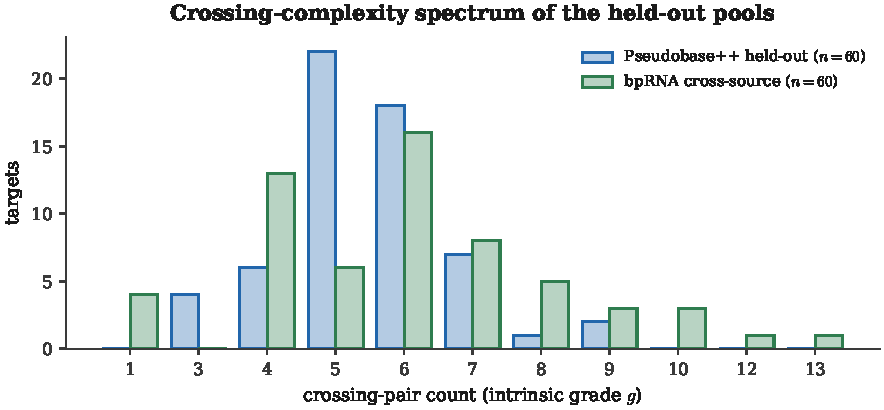
\includegraphics[width=0.82\linewidth]{fig_cc_grades.pdf}
\caption{Crossing-complexity spectrum (crossing-pair count $g$) of the primary Pseudobase++ held-out pool and
the independent bpRNA cross-source pool---overlapping ranges, so cross-dataset comparison is
grade-fair.}\label{fig:grades}
\end{figure}

\section{Full Experimental Results}\label{app:results}
Table~\ref{tab:appfull} collects every arm on every pool. Table~\ref{tab:appfamily} is the per-size family
sweep; Table~\ref{tab:appinvent} is the agent-invention trajectory.
\begin{table}[h]\centering\small
\setlength{\tabcolsep}{5pt}\renewcommand{\arraystretch}{1.15}
\caption{All arms $\times$ all pools. ``p-un.'' $=$ panel-unanimous (pKiss\,$\wedge$\,ProbKnot\,$\wedge$\,ShapeKnots,
exact). Floor $=$ \CF-confined REMC; gamer $=$ single-oracle (pKiss) operator; DesiRNA $=$ borrowed SOTA;
panel\_auto $=$ our two-oracle operator; agent $=$ the autonomously-written operator (App.~\ref{app:invent}).}\label{tab:appfull}
\begin{tabularx}{\linewidth}{@{}l >{\hsize=.92\hsize}X >{\hsize=1.08\hsize}X@{}}
\toprule
arm / pool & held-out primary ($n{=}60$) & other pools\\
\midrule
\CF{} floor & $0/60$ & $0/50$ (2nd); $0/60$ (cross); $0/10$ (family)\\
gamer (pKiss) & $43/60$ pKiss; $2/43$ ProbKnot; $1/60$ p-un. & ---\\
DesiRNA (borrowed) & $43/60$ pKiss; $26/43$ ProbKnot; $0/43$ p-un. & $2/10$ p-un. (family); $9/60$ pKiss, $0/60$ p-un. (cross)\\
panel\_auto (5 seeds) & pKiss$\wedge$ProbKnot $\{37,34,37,36,34\}$; p-un.\ $\{8,3,5,5,4\}$ (mean $5.0$) & $5/50$ p-un.\ (2nd); $2/60$ pk$\wedge$pb, $0/60$ p-un.\ (cross); $4/10$ p-un.\ (family)\\
\textbf{agent-invented} (6 models) & pKiss$\wedge$ProbKnot $26$--$42/60$; \textbf{p-un.\ $2$--$17/60$} (Table~\ref{tab:models}) & $4/6$ exceed hand-built; inherit cross-source narrowness\\
\bottomrule
\end{tabularx}
\end{table}
\begin{table}[h]\centering\small
\setlength{\tabcolsep}{5pt}\renewcommand{\arraystretch}{1.1}
\caption{Family $\mathcal L_{\mathrm H}$ sweep (Fig.~\ref{fig:family}). $\times$ = not realized; pk$\wedge$pb =
pKiss and ProbKnot; \textsc{u} = panel-unanimous.}\label{tab:appfamily}
\begin{tabularx}{\linewidth}{@{}lcccccccccc@{}}
\toprule
$n{=}m$ & 3 & 4 & 5 & 6 & 7 & 8 & (3,6) & (6,3) & (4,8) & (8,4)\\
\midrule
\CF{} floor & $\times$ & $\times$ & $\times$ & $\times$ & $\times$ & $\times$ & $\times$ & $\times$ & $\times$ & $\times$\\
DesiRNA & pk & pk & \textsc{u} & pk & \textsc{u} & pk & pk & pk & pk & pk\\
panel\_auto & pk$\wedge$pb & pk$\wedge$pb & \textsc{u} & \textsc{u} & \textsc{u} & pk$\wedge$pb & \textsc{u} & pk$\wedge$pb & pk$\wedge$pb & pk$\wedge$pb\\
\bottomrule
\end{tabularx}
\end{table}
\begin{table}[h]\centering\small
\setlength{\tabcolsep}{6pt}\renewcommand{\arraystretch}{1.1}
\caption{Autonomous invention trajectory (GLM-5.2, training pool $=$ Pseudobase idx $110$--$125$, disjoint
from held-out). Round $5$ failed to compile and was discarded; round $2$ (best) was frozen and
certified.}\label{tab:appinvent}
\begin{tabularx}{\linewidth}{@{}lccccccX@{}}
\toprule
round & 0 & 1 & 2 & 3 & 4 & 5 & frozen (round 2) on held-out $60$\\
\midrule
train solved $/16$ & 1 & 11 & \textbf{12} & 11 & 10 & --- & $35/60$ pKiss$\wedge$ProbKnot; $9/60$ panel-unanimous\\
\bottomrule
\end{tabularx}
\end{table}

\section{The Autonomous Operator-Invention Protocol}\label{app:invent}
\begin{figure}[h]\centering
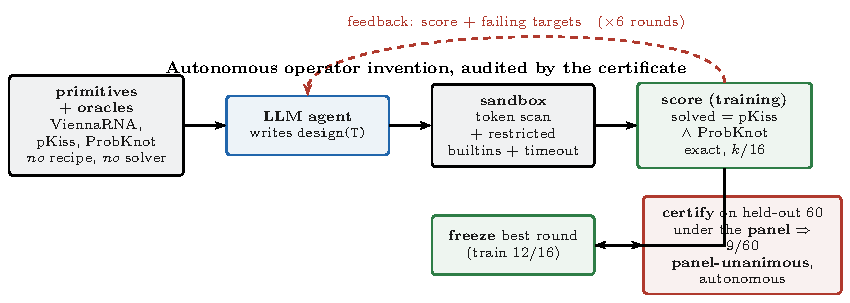
\includegraphics[width=0.99\linewidth]{fig_cc_invention.pdf}
\caption{The autonomous invention loop. The agent receives only primitives and the folding oracles---no
recipe, no external solver; each candidate is sandboxed and scored on a disjoint training pool; the score and
failing targets are fed back for six revision rounds; the best round is frozen and \emph{certified} by the
same panel used for the hand-built operators.}\label{fig:invention}
\end{figure}
An LLM agent (GLM-5.2, temperature $0.4$, no output cap) is given a documented \emph{primitive API}
and asked to write one function \texttt{design(target,seed)}; it may not import anything or call an external
pseudoknot solver. The primitives are: \texttt{fold\_cf} (ViennaRNA MFE, nested), \texttt{inverse\_fold\_cf}
(nested inverse fold), \texttt{fold\_pkiss\_pairs} and \texttt{fold\_probknot\_pairs} (the two crossing-aware
oracles, as pair sets), \texttt{target\_pairs} (parse a crossing dot-bracket), \texttt{rand\_seq}, and the
complement map; plus \texttt{random}/\texttt{math}/\texttt{itertools}. Each candidate is (i) scanned for
forbidden tokens (\texttt{import}, \texttt{os.}, \texttt{eval}, file/network, dunder access) and rejected if
present, (ii) \texttt{exec}'d with a restricted \texttt{\_\_builtins\_\_} whitelist, and (iii) run per target
under a \texttt{SIGALRM} wall-clock cap. It is scored on the disjoint training pool (solved $=$
pKiss\,$\wedge$\,ProbKnot exact), and the score plus failing examples are fed back for revision over six
rounds, carrying the full conversation. The best round is frozen and certified on the held-out $60$ under the
full panel; autonomy is structural (no solver is exposed). The agent independently converged on: split the
target into nested and crossing pairs; enforce Watson--Crick complementarity at paired positions; then greedily
mutate error positions to minimize a $\lvert T\!\setminus\!P_{\mathrm{pKiss}}\rvert + \lvert T\!\setminus\!P_{\mathrm{ProbKnot}}\rvert
+ 2(\lvert P_{\mathrm{pKiss}}\!\setminus\!T\rvert + \lvert P_{\mathrm{ProbKnot}}\!\setminus\!T\rvert)$ panel-agreement cost.
The invented source is archived at \texttt{runs/cc\_ascent/invent\_operator/invented\_design.py}.
Figure~\ref{fig:invent} shows the learning curve: the agent's training solve rate rises as it folds oracle
feedback into successive rewrites, and the frozen best round certifies at $9/60$ panel-unanimous on the
held-out pool. This is the worked example for one model; the analogous frozen results for all six frontier
models (three open, three closed) are summarized in Table~\ref{tab:models}, and every one peaks by round
$\le5$.

\begin{figure}[h]\centering
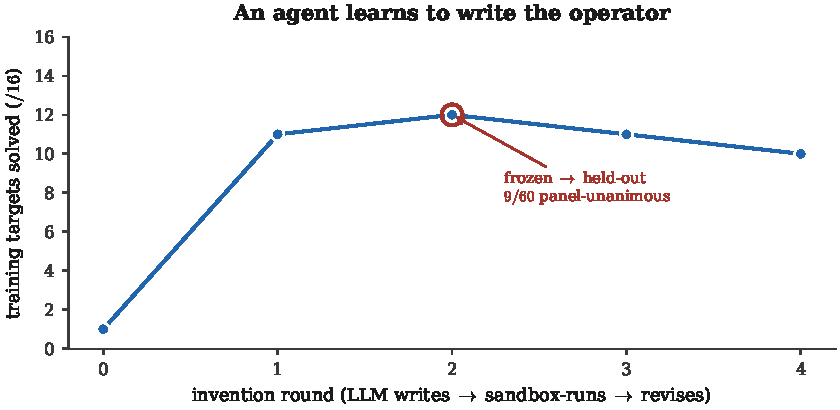
\includegraphics[width=0.78\linewidth]{fig_cc_invent.pdf}
\caption{The autonomous-invention loop learns. Training solve rate ($/16$, disjoint pool) across rounds as an
LLM agent writes, sandbox-runs, and revises a \texttt{design()} operator; the best round is frozen and
certified on the held-out $60$.}\label{fig:invent}
\end{figure}

\section{Oracle Configurations, Hyperparameters, Compute, and Verifier Stringency}\label{app:config}
\begin{table}[h]\centering\small
\setlength{\tabcolsep}{5pt}\renewcommand{\arraystretch}{1.15}
\caption{Oracle configurations. All deterministic and replayable; DATAPATH pinned to the RNAstructure data
tables.}\label{tab:appconfig}
\begin{tabularx}{\linewidth}{@{}lLll@{}}
\toprule
oracle & engine / mode & environment & timeout\\
\midrule
$\Omega_{\mathrm{cf}}$ & ViennaRNA, Turner-2004 MFE, $37^\circ$C & \texttt{rna} & --\\
pKiss (reference) & pKiss \texttt{mfe} \citep{janssen2015pkiss} & \texttt{pk} & $60$\,s\\
ProbKnot & RNAstructure MEA over the partition ensemble \citep{bellaousov2010probknot} & \texttt{rnastr} & $60$\,s\\
ShapeKnots & RNAstructure MFE-based, run \emph{de novo} (no SHAPE) \citep{hajdin2013shapeknots} & \texttt{rnastr} & $120$\,s\\
\bottomrule
\end{tabularx}
\end{table}
\noindent\textbf{Operator hyperparameters.} REMC floor: wall $30$\,s. Design operators (fixed across all
targets $=$ a uniform procedure): skeleton budget $12$--$20$\,s, repair budget $90$--$120$\,s, $\le800$--$1500$
repair iterations, ProbKnot gate at $\mathrm{pk\_bp}\le3$. \textbf{Compute.} A single $256$-core host;
target-level parallelism at $\mathrm{NWORKERS}{=}60$ (the design operators are single-process, so this is
safe); the entire sweep suite is search-only and incurs \emph{no} model-inference cost, except the invention
agent (App.~\ref{app:invent}), a few dollars of GLM-5.2.

\smallskip\noindent\textbf{Positive-side stringency (the verifier ladder).} The positive verdict is not
``the target pairs appear somewhere'': panel-unanimous requires the target to \emph{equal} each method's
predicted structure---the MFE under pKiss and ShapeKnots and the maximum-expected-accuracy structure over a
partition-function ensemble under ProbKnot---so it sits at the ``unique/dominant fold'' rung of the
exact\,$\subseteq$\,unique-MFE\,$\subseteq$\,dominance ladder of Fig.~\ref{fig:ladder}, agreed by three
independent engines. We \emph{climb one rung further and measure it} (\S\ref{sec:exp},
Fig.~\ref{fig:stringency}, \texttt{runs/cc\_ascent/positive\_stringency.py}): enumerating pKiss suboptimals for
the certified designs, the target is the pKiss MFE for all $17$ that enumerated within budget and is dominant
over the best alternative fold by a median $1.2$\,kcal/mol ($14/17$ clear $\ge1$\,kcal). The verdict remains
\emph{model-relative}---all engines are thermodynamic secondary-structure predictors, not physical ground
truth---and two further strengthenings are computable with the installed tooling (\texttt{partition},
\texttt{ProbabilityPlot}, \texttt{pKiss\_probs}): a Boltzmann-probability threshold and a fourth,
non-thermodynamic (learned) predictor. Physical confirmation (in-vitro probing, Fig.~\ref{fig:ladder} R4) is
the only route past model-relativity and is out of scope here.

\begin{figure}[h]\centering
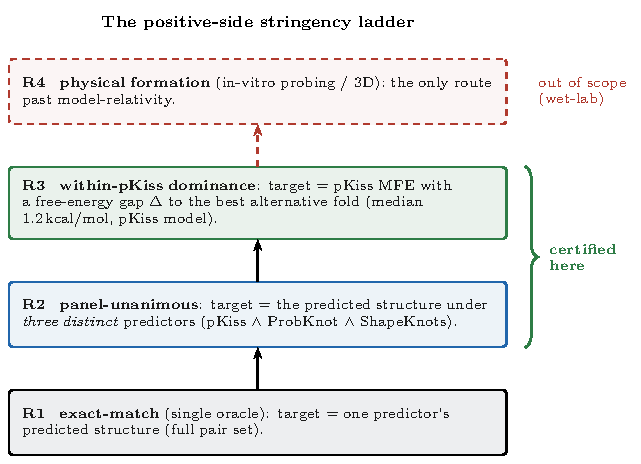
\includegraphics[width=0.66\linewidth]{fig_cc_ladder.pdf}
\caption{The positive-side stringency ladder. Panel-unanimity certifies at R2; the measured energy-gap
dominance (\S\ref{sec:exp}) is R3; R4 (physical formation) needs wet-lab and is out of scope.}\label{fig:ladder}
\end{figure}

\bibliographystyle{plainnat}
\bibliography{references}
\end{document}
